\documentclass[11pt]{article}
\usepackage[margin=1in]{geometry}
\usepackage{amsmath,amssymb,amsthm}
\usepackage{graphicx}
\usepackage{float}
\usepackage[onehalfspacing]{setspace}
\usepackage[unicode=true,
 bookmarks=true,bookmarksnumbered=false,bookmarksopen=false,
 breaklinks=false,pdfborder={0 0 0},pdfborderstyle={},backref=false,colorlinks=true]
 {hyperref}
\usepackage{verbatim}
\usepackage{appendix}
\usepackage{mathtools}
\usepackage{url}
\usepackage[authoryear]{natbib}
\usepackage{soul}
\usepackage{tikz}
\usepackage{booktabs} %Package with \toprule and \bottomrule
\usetikzlibrary{calc}
\usepackage{caption}
\usepackage{subcaption}
\usepackage{comment}
\usepackage{ulem}
\usepackage{setspace}
\usepackage[en-US]{datetime2}

\renewcommand{\v}[1]{\ensuremath{\mathbf{#1}}} % for vectors
\newcommand{\gv}[1]{\ensuremath{\mbox{\boldmath$ #1 $}}} 
% for vectors of Greek letters
\newcommand{\uv}[1]{\ensuremath{\mathbf{\hat{#1}}}} % for unit vector
\newcommand{\abs}[1]{\left| #1 \right|} % for absolute value
\newcommand{\avg}[1]{\left< #1 \right>} % for average
\let\underdot=\d % rename builtin command \d{} to \underdot{}
\renewcommand{\d}[2]{\frac{d #1}{d #2}} % for derivatives
\newcommand{\dd}[2]{\frac{d^2 #1}{d #2^2}} % for double derivatives
\newcommand{\pd}[2]{\frac{\partial #1}{\partial #2}} 
% for partial derivatives
\newcommand{\pdd}[2]{\frac{\partial^2 #1}{\partial #2^2}} 
% for double partial derivatives
\newcommand{\pdc}[3]{\left( \frac{\partial #1}{\partial #2}
 \right)_{#3}} % for thermodynamic partial derivatives
\newcommand{\ket}[1]{\left| #1 \right>} % for Dirac bras
\newcommand{\bra}[1]{\left< #1 \right|} % for Dirac kets
\newcommand{\braket}[2]{\left< #1 \vphantom{#2} \right|
 \left. #2 \vphantom{#1} \right>} % for Dirac brackets
\newcommand{\matrixel}[3]{\left< #1 \vphantom{#2#3} \right|
 #2 \left| #3 \vphantom{#1#2} \right>} % for Dirac matrix elements
\newcommand{\grad}[1]{\gv{\nabla} #1} % for gradient
\let\divsymb=\div % rename builtin command \div to \divsymb
\renewcommand{\div}[1]{\gv{\nabla} \cdot \v{#1}} % for divergence
\newcommand{\curl}[1]{\gv{\nabla} \times \v{#1}} % for curl
\newcommand{\stkout}[1]{\ifmmode\text{\sout{\ensuremath{#1}}}\else\sout{#1}\fi}
\newcommand{\msout}[1]{\text{\sout{\ensuremath{#1}}}}
\let\baraccent=\= % rename builtin command \= to \baraccent
\renewcommand{\=}[1]{\stackrel{#1}{=}} % for putting numbers above =
\providecommand{\wave}[1]{\v{\tilde{#1}}}
\providecommand{\fr}{\frac}
\providecommand{\RR}{\mathbb{R}}
\providecommand{\NN}{\mathbb{N}}
\providecommand{\seq}{\subseteq}
\providecommand{\e}{\epsilon}
\newtheorem{prop}{Proposition}
\newtheorem*{lem}{Lemma}
\theoremstyle{definition}
\newtheorem*{dfn}{Definition}
\newenvironment{s}{%\small%
        \begin{trivlist} \item \textbf{Solution}. }{%
            \hspace*{\fill} $\blacksquare$\end{trivlist}}%
\newenvironment{p}{}{}
\DeclareMathOperator*{\argmax}{arg\,max}
\DeclareMathOperator*{\argmin}{arg\,min}

\hypersetup{
	pdftex,
    pdfauthor={Jonathan I. Dingel and friends},     % author
    colorlinks=true,       % false: boxed links; true: colored links
    linkcolor=red,          % color of internal links
    citecolor=black,        % color of links to bibliography
    urlcolor=blue           % color of external links
}

% CUSTOM DEFINITIONS
\urldef{\dingelhomepage}\url{http://faculty.chicagobooth.edu/jonathan.dingel/}
\urldef{\rufemail}\url{jcruf@uchicago.edu}
\newtheorem{proposition}{Proposition}

% IDENTIFYING INFORMATION
\title{Machine Politics in Chicago's Menu Program\thanks{
	I thank Jonathan Dingel, Anthony Fowler, Thomas Malthouse, and the participants of the 2022 UChicago RP Workshop for their helpful comments and suggestions. \rufemail
}}
\author{John C. Ruf}
\date{\today}


\begin{document}
\bibliographystyle{../bib/aeanobold}
\maketitle
% -----------------------------------------------
% 	ABSTRACT
% -----------------------------------------------

\begin{abstract}
\begin{spacing}{1.0}
This paper investigates the political economy of conspicuous public spending. 
It defines conspicuous public spending as spending intended to signal competency to voters for electoral gain. 
A simple career-concerns model featuring a tradeoff between conspicuous and inconspicuous expenditures with experience gain demonstrates this effect in a rational-choice framework. 
The model has two critical implications. 
Firstly, unexpected increases in conspicuous expenditures help politicians get re-elected. 
Secondly, less-experienced politicians spend more conspicuously than their established counterparts. 
This paper uses data from Chicago's Aldermanic Menu Program to test these implications. 
The first implication is confirmed via a simple discrete-choice analysis. Differences-in-differences methods further show some evidence for the second implication. 
However, counter to the model, the Differences-in-Differences study shows an effect that decays before the next election.
Furthermore, a regression discontinuity analysis also shows an increase in spending, which is not consistent with the model.
This paper concludes by exploring alternative hypotheses that may be driving the decaying effect.
\end{spacing}
\end{abstract}
\vspace{1cm}
{\small
\noindent \textit{Keywords}: Menu Program, Aldermen, Infrastructure Maintenance, Local Politics, Spatial Distribution, Machine Politics  \\
\textit{JEL codes}: H41 H72 L98 
}
\thispagestyle{empty}
\newpage
\setcounter{page}{1}

% -----------------------------------------------
% 	BODY
% -----------------------------------------------

%\section{Introduction}

\begin{frame}{Motivation}
    How do local politicians allocate infrastructure maintenance and other key public goods?
    \begin{itemize}
        \item (Glaeser 2019) find a strong shortage of road maintenance in the country: is it a political economy problem?
        \item If local politicians cannot be trusted to maintain key infrastructure and roads, that has important welfare implications for optimal placement of ``large'' welfare enhancing projects.
        \item How prevalent would clientelism be if we allocated public resources in a more decentralized manner?
        \item What are the costs of giving local politicians unilateral control over infrastructure maintenance? What magnitude would the benefits like ``local knowledge'' and ``accountability'' need to be to justify this?
    \end{itemize}
\end{frame}
    
\begin{frame}{What do aldermen do?}
    \begin{center}
    \begin{quotation}
        ``I remember crossing California going west, every street was resurfaced almost every year. They always had brand new lighting and then east of California, where Ald. Bernie Stone would lose the precincts consistently, I mean the streets were in shambles.'' \\
    \end{quotation}
    \end{center}
    \raggedleft{ -Ald. Carlos Ramirez-Rosa (35th Ward).}
    \begin{itemize}
        \item Aldermen as Mini-Mayor over Ward
        \begin{itemize}
            \item City council defers to Ward Alderman all internal issues
            \item Eg. \ snow plows, garbage cleanup, sign permits, business licenses, liquor-moratoriums, and of course, construction and zoning.
            \item A relatively new power that aldermen were granted in 1995 is the ability to allocate \$1.5M in infrastructure ``menu'' requests 
        \end{itemize}
    \end{itemize}
\end{frame}
    
\begin{frame}{What is the Aldermanic Menu Program?}
        Alderman have the power to allocate \$ 1.5M on a variety of infrastructure projects. They are given a map of 311 complaints for guidance.
    \begin{itemize}
        \item  5 primary categories:
        \begin{itemize}
            \item \textbf{Streets/CDOT:} Alley/Road/Sidewalk Resurfacing, speed bump replacement, sign installation, Curb and Gutter fixes, etc. 
            \item \textbf{Crime Prevention and Lighting:} Camera installation and street lights
            \item \textbf{Arts:} Murals and Neighborhood Arts programs
            \item \textbf{Schools:} Direct grants to CPS, Sports Fields, Gardens, Auditoriums, Playgrounds, etc. 
            \item \textbf{Parks, Trees, and Gardens:} Tree planting, public garden formation, and park cleanup programs. 
        \end{itemize}
    \end{itemize}
\end{frame}

\begin{frame}{2017 OIG Audit}
        The office of the inspector general (OIG) conducted an audit of the menu program in 2017.
        The audit was scathing. 
        They recommended dismantling the program and reallocating the funds to a more traditional central planning model.
        The primary findings of the audit are given below.
    \begin{enumerate}
        \item  Menu, which serves as the City's primary residential infrastructure
        program, underfunds residential infrastructure needs and results in
        significant funding disparities relative to need between wards.
        \item   In the years 2012 through 2015, the City permitted aldermen to designate
        \$15.1 million of Menu funds for projects unrelated to core residential
        infrastructure.
        \item CDOT allowed at least \$825,292 in Menu spending on projects falling outside
        the appropriate ward boundaries and did not enforce project selection
        submission deadlines.
    \end{enumerate}
\end{frame}
%\input{./sections/theory.tex}
%\input{./sections/estimation.tex}
%\input{./sections/discussion.tex}
\section{Introduction}\label{sec:Introduction}

Do local politicians use machine-style politics to drive public goods towards their supporters? Is spending bias exacerbated or curbed by local political competition?
Because most municipalities allocate spending through collective decision-making bodies such as councils, it is usually difficult to attribute expenditures to individual politicians.
However, one such program exists in the United States: Chicago's Aldermanic Menu Program.
Through this program, the Chicago Department of Transportation (CDOT) gives each of Chicago's 50 aldermen a \$1.5 million budget, an eponymous ``menu'' of common expenditures, and a map of 311 complaints in their ward.
Using these resources, aldermen allocate funds to infrastructure maintenance, parks, and other public goods within their wards, even if they are not on the ``menu.''

This paper asks whether the menu funding towards each alderman's supporters or detractors changes after the alderman leaves office.
If so, what determines the magnitude of this change? 
To answer this, this paper uses a differences-in-differences design to compare the time trends of each supporting or opposing precinct before and after the alderman leaves office.
There are two cases where parallel trends are likely to hold: in close elections where the incumbent wins by a small margin and in cases where the incumbent is indicted and forced to leave office.
In the former, both wards where the aldermen just barely won and just barely lost should have similar spending trends.
Furthermore, both winning and losing aldermen in these cases should have similar expectations of winning, so they should behave similarly in the run-up to the election.
In the latter, the timing of the in-office indictment is uncertain, so 


This paper makes two contributions, firstly it publicly introduces this setting's data, and secondly it finds cases that supports \cite{dixit_londregan1996}'s theory of machine politics.
\cite{dixit_londregan1996} argue that the key to machine politics is for politicians to be more efficient at allocating public goods to their supporters than their opponents.
If this is the case, then the municipality arrives at a ``machine politics'' equilibrium where the incumbent targets all publics goods to their top supporters.
If there is no particular efficiency towards supporters, the municipality goes to a ``downsian'' equilibrium where both the incumbent and the challenger promise to allocate public goods to the most marginal voters.
This paper offers the first quantitative proof of the rumor that Bernie Stone biasedly allocating his funds.
It shows a large swing in fund allocation to the lowest and highest 20\% of precincts by campaign contributions before and after Stone's 2011 defeat by Debra Silverstein. 
Post-defeat, the bottom 20\% precincts saw a \$20,000 yearly increase in funds, while the top 20\% precincts experienced a decline nearly double of that.
This constitutes a difference of 1.65\% of the budget, or \$21,383 per year.
Finally, the paper finds that the stone case study is not always generalizable to other aldermen.
When examining close elections, the paper finds no significant difference in spending trends between the winning and losing aldermen.
However, when looking at aldermen who retire after being indicted, precincts that supported an indicted alderman saw their budget fraction decrease by 1.14pp after his/her removal from office, while those that did not saw a 2.59pp increase, amounting to a total difference of \$56,000 difference each year between the two groups.


Section~\ref{sec:background} describes the program's history, its rules, and its 2017 audit.
Section~\ref{sec:lit_review} describes the public economics literature on public goods allocation and lobbying and the spatial and urban economics literature on infrastructure allocation and how this paper relates to both literatures.
Section~\ref{sec:data_description} describes how the menu program data was collected, its summary statistics, and depicts an aggregate map of menu spending across Chicago for the past decade.
Section~\ref{sec:case_study} presents descriptive data for the case study of Alderman Bernie Stone, rumored to favor supporters with menu program funds. 
Section~\ref{sec:empframe} explains this paper's empirical strategy to determine if the Stone case study can be generalized to other aldermen.
Section~\ref{sec:results} shows the results of said empirical strategy, which finds that aldermen removed or retired due to criminal indictments, which has similar results to the Stone case study. 
However, this does not generalize to competitive elections.
The results from the indictment-based differences-in-differences design are statistically weak and sensitive to the number of precincts included, but are economically large and significant.
Section~\ref{sec:conclusions} concludes.


\section{Background}\label{sec:background}

The aldermanic menu program was initiated in 1994 and continues to this day \citep{OIGaudit}. 
The program delegates approximately \$75 million every year to be split equally amongst the 50 aldermen in Chicago's city council to be spent on projects they unilaterally select for their ward, given a ``menu'' of acceptable expenditures. 
Each alderman allocates approximately \$1.5 million per year to their ward.
Chicago's Office of Budget and Management (OBM) tracks the spending and its Department of Transportation (CDOT) manages the program.
Each ward is defined to be approximately equal by population every 10 years, depending on the decennial census results, but the overall map is subject to a city council vote for approval.
The Chicago Board of Elections draws the precinct map using the ward map, according to the available number of polling places, and each contain between 500 to 800 voters \citep{Crowley_2022}.
Each year in the spring, the Mayor, CDOT, and OBM send letters to the aldermen explaining the program and providing a menu of cost estimates and a list of possible projects.
Before the aldermen select projects, CDOT and OBM provide a briefing packet with 311 complaint data.
Finally, aldermen more or less spend the money as they see fit, with the only hard restriction being that they cannot spend more than \$1.32 million on any one project.
Because this program and elections occur in the spring, new aldermen can only spend their entire menu funds the following year and often rely on the previous Alderman's programmed budget the year they are elected.

``Off-menu'' expenditures are also allowed, of which most ``off-menu'' funds go towards Parks, Chicago Public Schools, and miscellaneous beautification projects such as trees, murals, decorative garbage cans, designer bike racks, and more \citep{OIGaudit}. 
While on-menu items are typically also provided by other funding sources within Chicago's Capital Improvement Program, off-menu items such as murals and statues are usually directly credited to the aldermen, thus giving an incentive to reward supporters' loyalty with public goods.
The program is unique insofar as it gives elected politicians a wide berth over a significant portion of the City's infrastructure budget and allows its use for items one does not typically think of as core infrastructure. 
An example of a portion of a menu from 2013 is shown below in Figure~\ref{fig:menu_example}.


\begin{figure}[H]
    \centering
    \caption{An Example of a menu from 2012/2013}\label{fig:menu_example}
    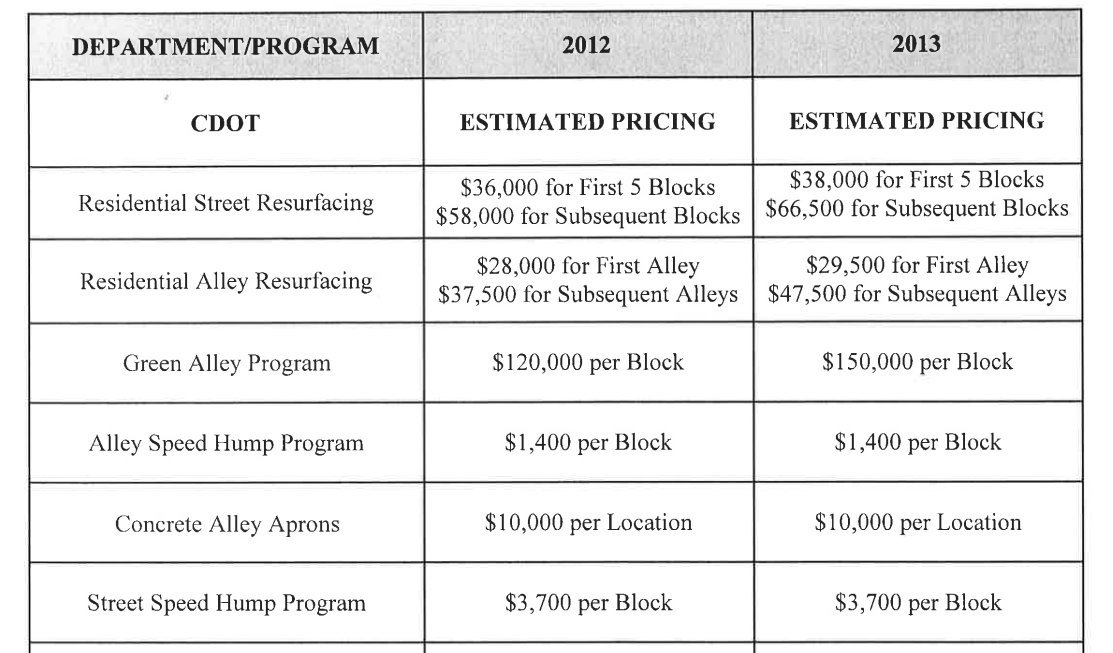
\includegraphics[scale=0.38]{input/menu_example.png}
\end{figure}

The Chicago Office of the Inspector General audited the program in 2017 and found that the program was rife with misallocation -- because wards are defined to be approximately equal by population but not equal by infrastructure needs, so some dense wards get 80\% or more of their needs met while others get only 10\% or less \citep{OIGaudit}.


Thus, the OIG found that the program resulted in significant funding disparities between wards relative to infrastructure needs.
Secondly, the OIG audit found that from 2012 through 2015, the program permitted aldermen to use \$ 15.1 million in menu funds for projects unrelated to so-called ``core'' infrastructure.
Finally, the OIG audit found that CDOT allowed aldermen to use \$825,292 of menu funds on projects outside of the ward they were elected to represent so that they could spend it on the wards they were running for reelection in.

\section{Literature Review}\label{sec:lit_review}

Most literature on political allocation of public goods in political economy focuses intently on theoretical models to explain behavior but comparatively little empirical testing of that behavior. 
This literature looks primarily at the political incentives to redistribute.
The early literature in political economy focused on variations of targetting the median voter, the seminal paper being \cite{downs1957economic}.
This earlier literature was largely successful in explaining platform convergence in two-party systems.
However, many political scientists and historians found this model wanting in addressing obvious cases of machine politics \cite{rakove1975don} \cite{golway2014machine}.
The harsh examples of the New York City Tammany Hall machine and the Chicago Democratic Machine are puzzling in a downsian framework, as they maintained power through tight control of patronage jobs and distributing public goods to reward supporters.
The resolution to this puzzle came in \cite{dixit_londregan1996}, which develops a general model of politics that encompasses both the median voter and patronage models.
The model they use matches the Chicago setting to a tee: they assume that politicians have a fixed budget to allocate to public goods and can distribute it to pressure groups to maximize their vote share.
In that model they find two equilibria: one where politicians allocate to supporters and one to marginal voters.
The critical difference between the two is whether or not the politician's spending is more effective on supporters. 
If a politician has specific ties that allow them to distribute more benefits at a lower cost to supporters, they will allocate to supporters.
This difference drives our choice of estimator, as this rules out some traditional continuous-treatment tools. 

In addition, this paper is related to the lobbying literature, which studies how special interest groups influence policy. 
The key paper in this literature is \cite{grossman_helpman_1994}, which develops a model of lobbying where firms can lobby politicians to influence policy that is determined by seats in a legislature. 
Their model finds that the party expected to win will cater more towards special interests.

Numerous empirical papers look at the political allocation of public goods.
For example, \cite{finan2021electoral}'s study looks at the allocation of funds from Brazil's federal legislature, where similarly, each of the 513 legislators in Brazil receives a fixed budget of BRL\$1.5 million each year for similar public infrastructure projects.  
Furthermore, electoral competition in Brazil is intense: Only 75\% of legislators even choose to run for reelection compared to Chicago's city council's actual reelection rate of 87\%.
Furthermore, incumbents can be challenged by other incumbents due to overlapping districts, whereas in Chicago, this problem only rarely happens when wards are redrawn.
In this paper, Finan and Mazzocco estimate a structural model to find that 26\% of public funds are distorted relative to a social planner's allocation. 
After estimating their structural model, they also found that implementing an approval voting system would reduce the distortions by 7.5\%. 
They also find that term limits may reduce distortion but increase corruption.
In addition, there is \cite{frank_hoopes_lester_2022} find that governors in the US select place-based tax incentive locations more often when the tract's state representative is a member of the governor's party and is greatest with Republican governors.
However, this paper borrows the most from the \cite{fowleretalquidproquo} study, which uses a combination of regression discontinuity and first-differences design to study whether there is evidence of successful corporate campaign contributions influencing the stock prices of the donors. 
From this two-pronged approach, Fowler et al. found that there really is no impact of a preferred candidate on winning, and thus, it is hard to argue that campaign contributions are a profitable venture for companies. 

This study is different from traditional political economy studies as it focuses on a municipal environment where the public good at play is primarily infrastructure. 
Thus, it is also related to the literature on municipal infrastructure provision and the new quantitative spatial economics literature.
This includes \cite{Glaeser2018political}, \cite{Fajgelbaum2023}, \cite{treb_arkolakis_2022_infrastructure}, and \cite{bordeu2023commuting}.
Glaeser's seminal paper focuses on infrastructure's ``visible'' and ``invisible'' effects. 
In particular, he finds that governments spend too much on new infrastructure projects and not enough on maintenance.
Furthermore, local voters are less likely to support new projects due to noise, land use, and other externalities from new construction.
Glaeser uses this framework to explain the decline of urban mega-projects.
Our framework differs as we look at the allocation of relatively low-nuisance maintenance and public goods projects rather than new construction.
Thus, we see the opposite problem in maintenance: electoral concerns lead to too much spending on supporters and not enough on the rest of the municipality.
Fajgelbaum et al. examine how political economy influenced the planning of California's high-speed rail (CHSR) project.
They find that preferences for widespread approval lead to the planner placing CHSR stations farther from dense metro areas than a politically blind planner.
Treb and Arkolakis' paper uses a quantitative spatial model to evaluate the impact of improving any segment of the infrastructure network on the entire network's welfare and finds in an empirical application that there are highly variable returns to investment across different links in the network.
Finally, Bordeu looks at how infrastructure is allocated across a similarly decentralized city, Santiago, Chile, and finds that the sub-city municipalities over-invest in core areas and under-invest in areas near their boundary using a quantitative spatial model.
This misallocation results in higher-cross-jurisdiction commuting costs, less concentrated employment, and a more comprehensive spatial distribution of production.
She finds that infrastructure centralization would increase aggregate infrastructure investment and population and yield large welfare gains.
\section*{Data}
The first data-set employed is web-scraped Aldermanic voting data. This data set contains 123 observations of determining election outcomes. 
Determining election indicates that an election determined who got the office. 
We remove elections where the general election outcome became a runoff to avoid double-counting. 
For the discrete-choice modeling, we use a reduced form of the Aldermanic voting data, with only observations from 2015 and 2019, so we have data on off-menu expenditures from the year before the election. 
Secondly, there are Aldermanic menu expenditures, which contain the yearly allotted allocations from Aldermen and their respective locations from 2012 to 2020. 
This data set contains 450 ward-year observations of the amount of money spent on off-menu items and on-menu items. 
For the DiD analysis, we will use the entire 450 observation data set, but for the regression discontinuity study, we will use only the 123 observations that correspond to the year after an election. 
This data-set comes from the Office of Budget and Management of the city of Chicago \cite{MenuProgramChoices}. 

The data set employed for the regression discontinuity analysis consists of 123 electoral observations across three elections. 
We can see a large standard deviation of off-menu expenditures consisting of approximately 10\% of the budget each alder-person is allocated. 
Furthermore, we can see that, on average, we expect the electoral outcomes of these contests to be heavily skewed towards the incumbent, with an average incumbent vote share of 65.5\%The summary stats for the regression discontinuity is below:

\begin{table}[H] \centering 
  \caption{Summary Statistics for the Regression Discontinuity Analysis} 
  \label{} 
\begin{tabular}{@{\extracolsep{5pt}}lccccc} 
\\[-1.8ex]\hline 
\hline \\[-1.8ex] 
Statistic & \multicolumn{1}{c}{N} & \multicolumn{1}{c}{Mean} & \multicolumn{1}{c}{St. Dev.} & \multicolumn{1}{c}{Min} & \multicolumn{1}{c}{Max} \\ 
\hline \\[-1.8ex] 
off\_menu & 123 & 48,775.410 & 118,910.400 & 0.000 & 705,155.000 \\ 
votepct & 123 & 65.546 & 17.628 & 32.262 & 100.000 \\ 
\hline \\[-1.8ex] 
\end{tabular} 
\end{table} 

The histogram of off-menu expenditures data employed in the regression discontinuity is below. 
In this, we see that the vast majority of wards spend \$0 on off-menu items, but a small minority of alderpersons seem to use off-menu expenditures. 
We also see that the right tail of the distribution is quite long, so not only are off-menu expenditures rare, but the ward may be spending a large amount of money when they happen.

\begin{figure}[H]
    \centering
    \includegraphics{figures/rdd_expenditures_histogram.png}
    \caption{Histogram of Off-Menu expenditures in 2012, 2016, and 2020 for the RD Analysis}
    \label{fig:my_label}
\end{figure}

A histogram of incumbent vote-shares used in the regression discontinuity analysis is shown below. 
Here we see that the distribution is quite irregular, featuring what seems to be a large discontinuity at the cutoff of 50\% with large density discontinuities elsewhere. 
The histogram shows that the data does not easily fit into a, say, a normal or some other kind of distribution. 
This is likely a reflection of the low number of observations as much as anything else.  

\begin{figure}[H]
    \centering
    \includegraphics{figures/rdd_votepct_histogram.png}
    \caption{Histogram of Incumbent Voteshares in 2011, 2015, and 2019 for the RD analysis}
    \label{fig:my_label}
\end{figure}

The Differences-in-differences data set comprises 450 observations of off-menu expenditures across 50 wards over nine years from 2012-2020. 
Twelve wards are "treated" with a leaving incumbent, of which six lost the election, and six retired \cite{election_results}. 
From the summary statistics of the data below, we can see that the treatment group makes up approximately a quarter of the data set and that average off-menu expenditures are lower in the group of wards that had an alderman retire or defeated in a reelection attempt. 

\begin{table}[H] \centering 
  \caption{Summary Statistics for Diff-in-Diff Analysis} 
  \label{} 
\begin{tabular}{@{\extracolsep{5pt}} cccccc} 
\\[-1.8ex]\hline 
\hline \\[-1.8ex] 
 Treatment Group & N & Mean & St. Dev & Min & Max \\ 
\hline \\[-1.8ex] 
treated & 108 & 38554.80 & 94170.02 & 0 & 550000 \\ 
untreated & 342 & 66857.15 & 129705.34 & 0 & 705155 \\ 
\hline \\[-1.8ex] 
\end{tabular} 
\end{table} 


A histogram is presented below for the off-menu expenditures featured in the figure below. 
From this, we can see that the data is similar to the regression discontinuity data set. 
There is a long right tail; most observations are clustered around or directly at zero. 

\begin{figure}[H]
    \centering
    \includegraphics{figures/did_hist.png}
    \caption{Off-Menu Expenditures per Unit Year for the Diff-in-Diff Analysis}
    \label{fig:my_label}
\end{figure}


\section{Bernie Stone Case Study}\label{sec:case_study}
This section discusses the Bernie Stone case study, which is the primary motivation for this paper.
Bernie Stone was an alderman in Chicago's 50th ward from 1973 to 2011.
He was well known for his, ``political philosophy.''

\begin{quotation}
    ``You take care of the people who take care of you — you know, the people who voted for you, That’s not Chicago politics, that’s Politics 101.'' - Alderman Bernie Stone (50th ward), Quoted from~\cite{BGA_berniequote}
\end{quotation}

In fact an alderman who grew up in the 50th ward once remarked that,

\begin{quotation}
    ``Well, I grew up in the 50th Ward and you know, God bless [the late former Ald.] Bernie Stone, may he rest in peace, but I remember crossing California going west, every street was resurfaced almost every year. They always had brand new lighting and then east of California, where he would lose the precincts consistently, I mean the streets were in shambles. Many people felt he was spending the bulk of the menu money west of California, where he was getting the bulk of the vote.'' - Alderman Carlos Ramirez-Rosa (35th Ward), Quoted from~\cite{ramirezrosaquote}
\end{quotation}

This quote is a clear example of the type of behavior that this paper seeks to investigate.
This phenomenon could not be verified previously because the CDOT did not make the 2005-2011 documents publicly available. 
Furthermore, the 2011-2022 data was in PDF form, making locating the spending tedious and difficult.
This paper is the first to put numbers to this anecdotal evidence.
First, we can look at a map of the precincts that supported Stone financially and electorally.
Below in Figure~\ref{fig:stone_support_maps}, we can see the precincts that supported Stone in the 2007 runoff election and the precincts that gave Stone the most individual contributions.
In both maps, we can see that the southwestern portion of the ward is the most supportive of Stone, on average.
\begin{figure}[H]
    \centering
    % First subfigure
    \begin{subfigure}[b]{0.45\textwidth} % [b] aligns at the bottom
    \includegraphics[width=\textwidth]{input/contribution_map_stone_ward_50_2003_2011.png}
    \caption{Campaign contributions to Alderman Stone, 2003-2011}
    \end{subfigure}
    \hfill % This adds some space between the two subfigures
    % Second subfigure
    \begin{subfigure}[b]{0.45\textwidth}
    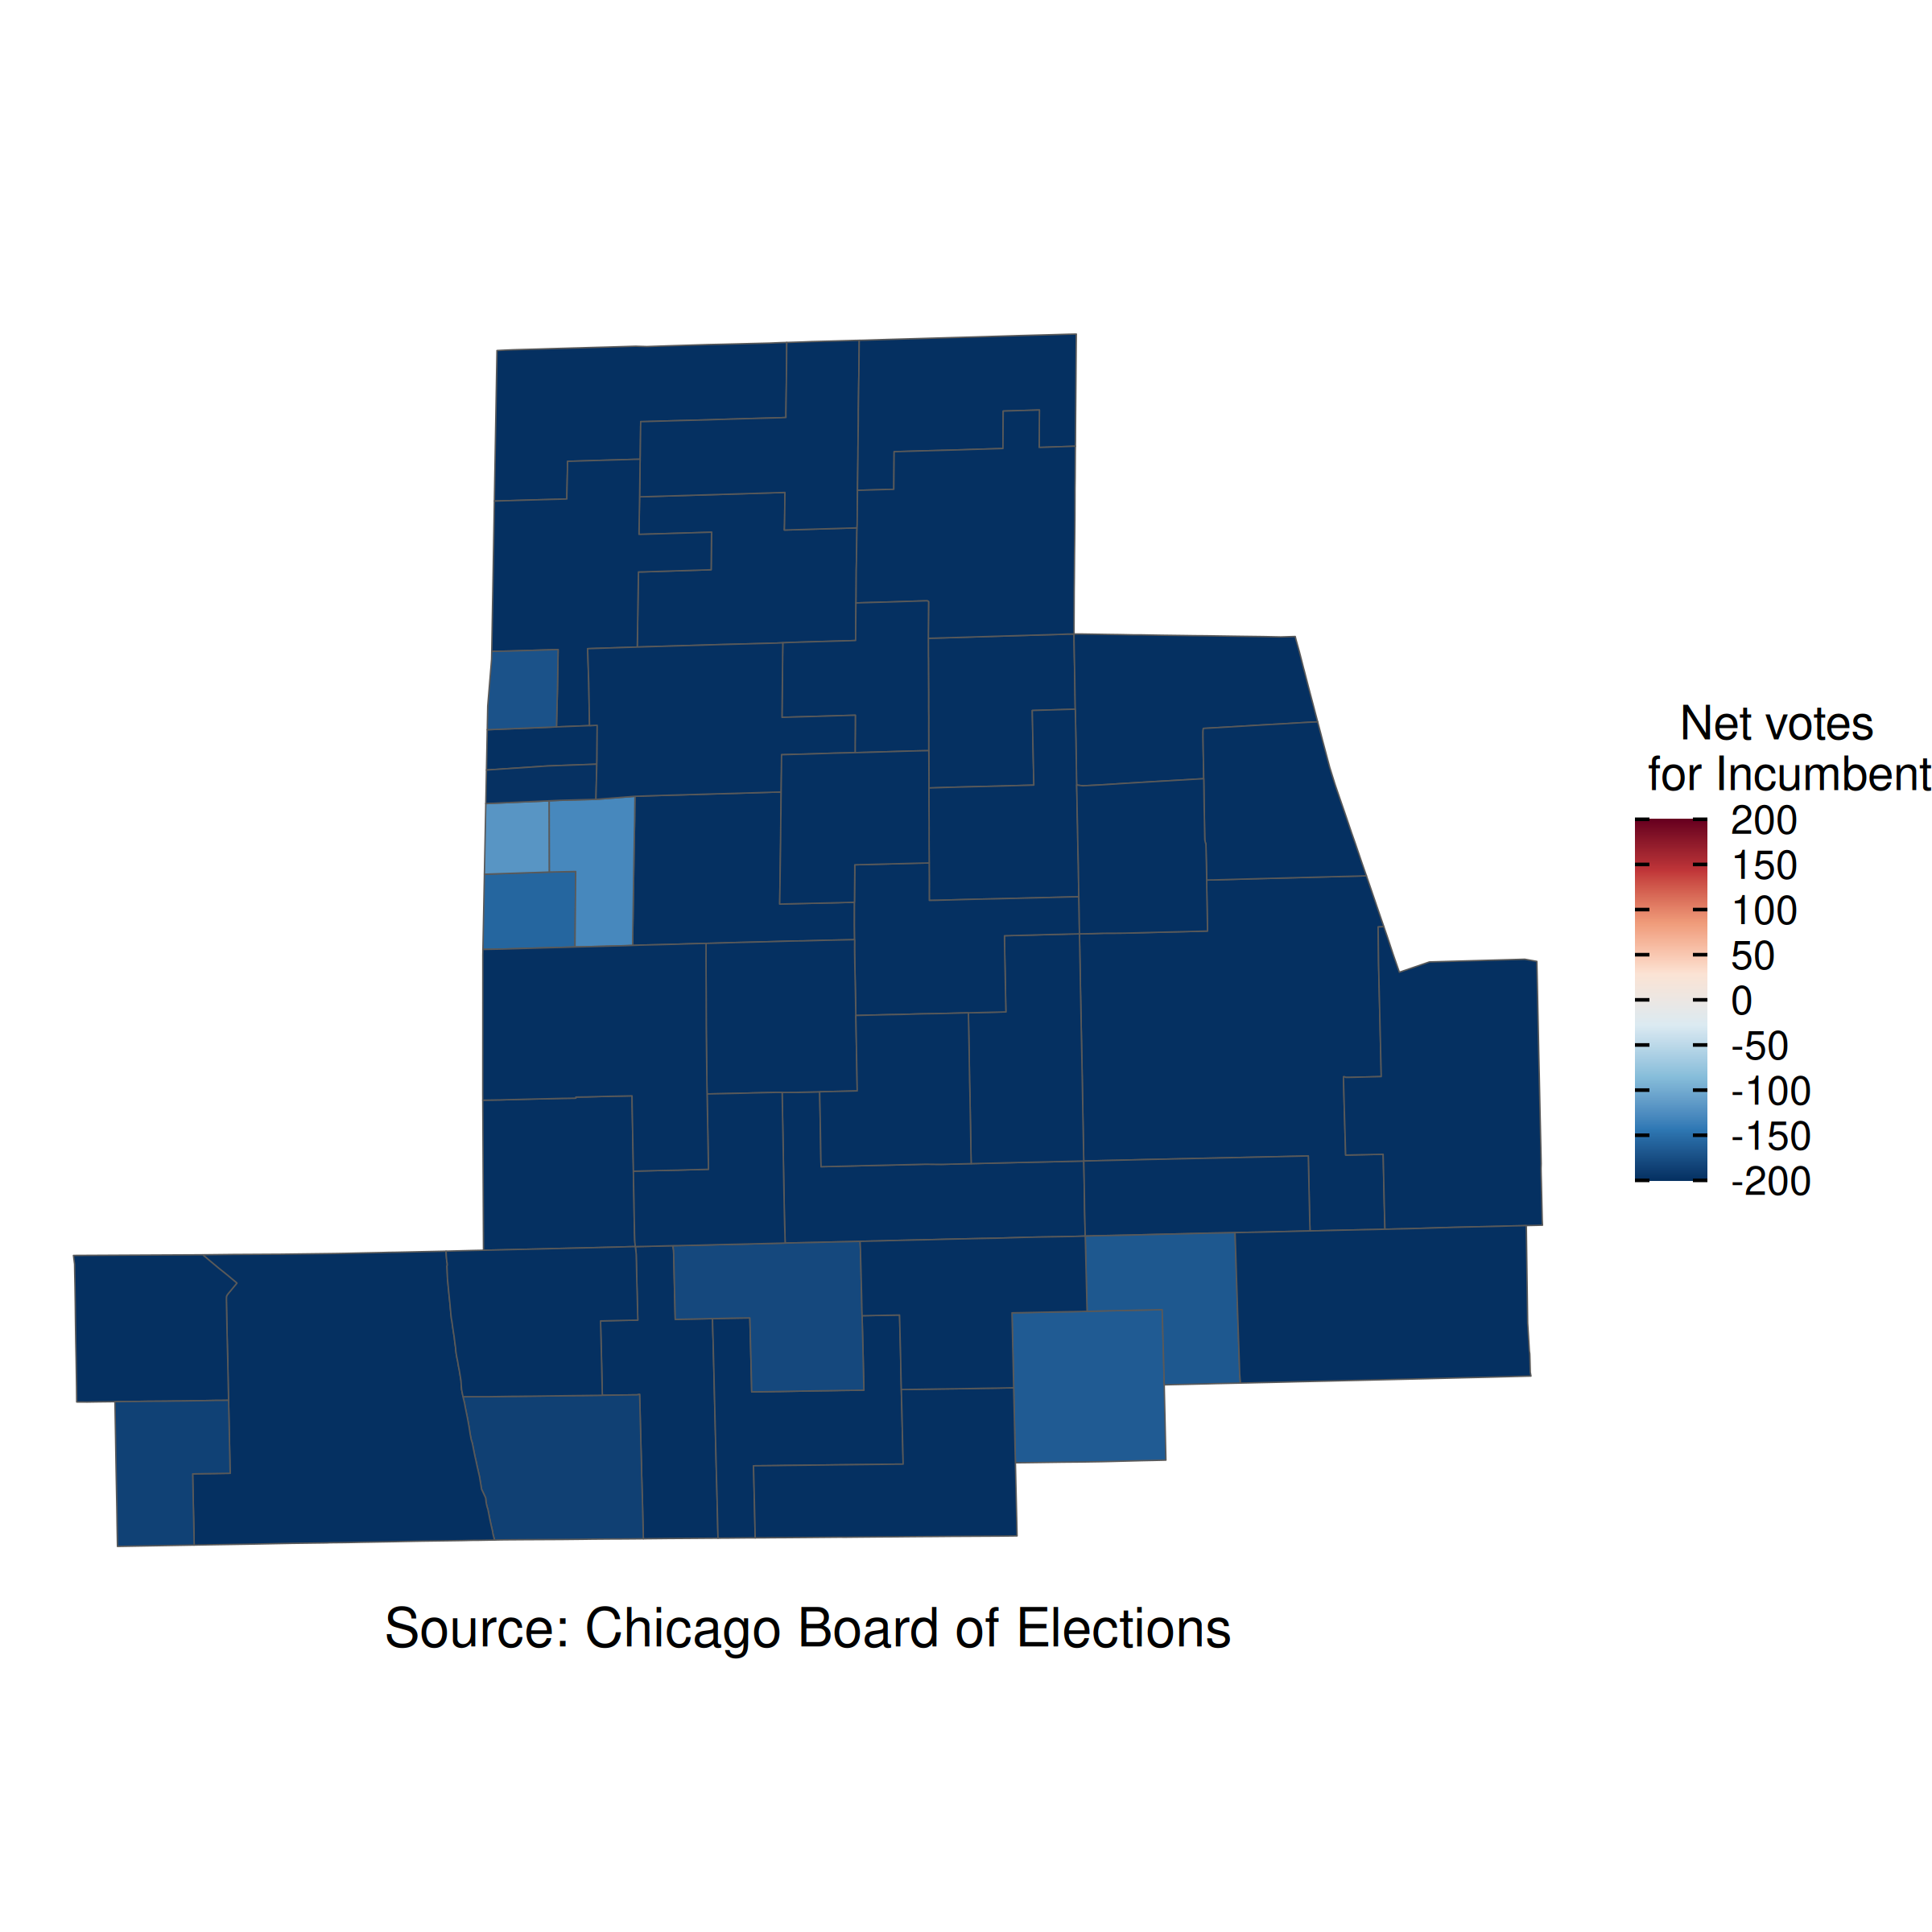
\includegraphics[width=\textwidth]{input/ward_50_2007_runoff_incumbent_precinct_results.png}
    \caption{Net votes for Alderman Stone, 2007}
    \end{subfigure}
    \caption{Distribution of Spending per Precinct for both ward maps in the dataset}
    \label{fig:stone_support_maps}
\end{figure}

Next, we can look at a time series of the spending per precinct for the 50th ward. 
There are approximately 44 precincts in the 50th ward, so Figure~\ref{fig:stone_spending_timeline} gathers the top and bottom quintile of precincts by contributions to Stone and shows the average fraction of the total located budget spent in each quintile. 
``other'' refers to all other precincts.
Note that the precincts that contributed the most to Stone's campaign are the same precincts that contributed the most net votes to Stone in the 2007 runoff election.
We see that after his reelection in 2007, Stone's spending per precinct was heavily concentrated in the precincts that supported him.
After his defeat, spending per precinct is much more evenly distributed across the ward.

\begin{figure}[H]
    \centering
    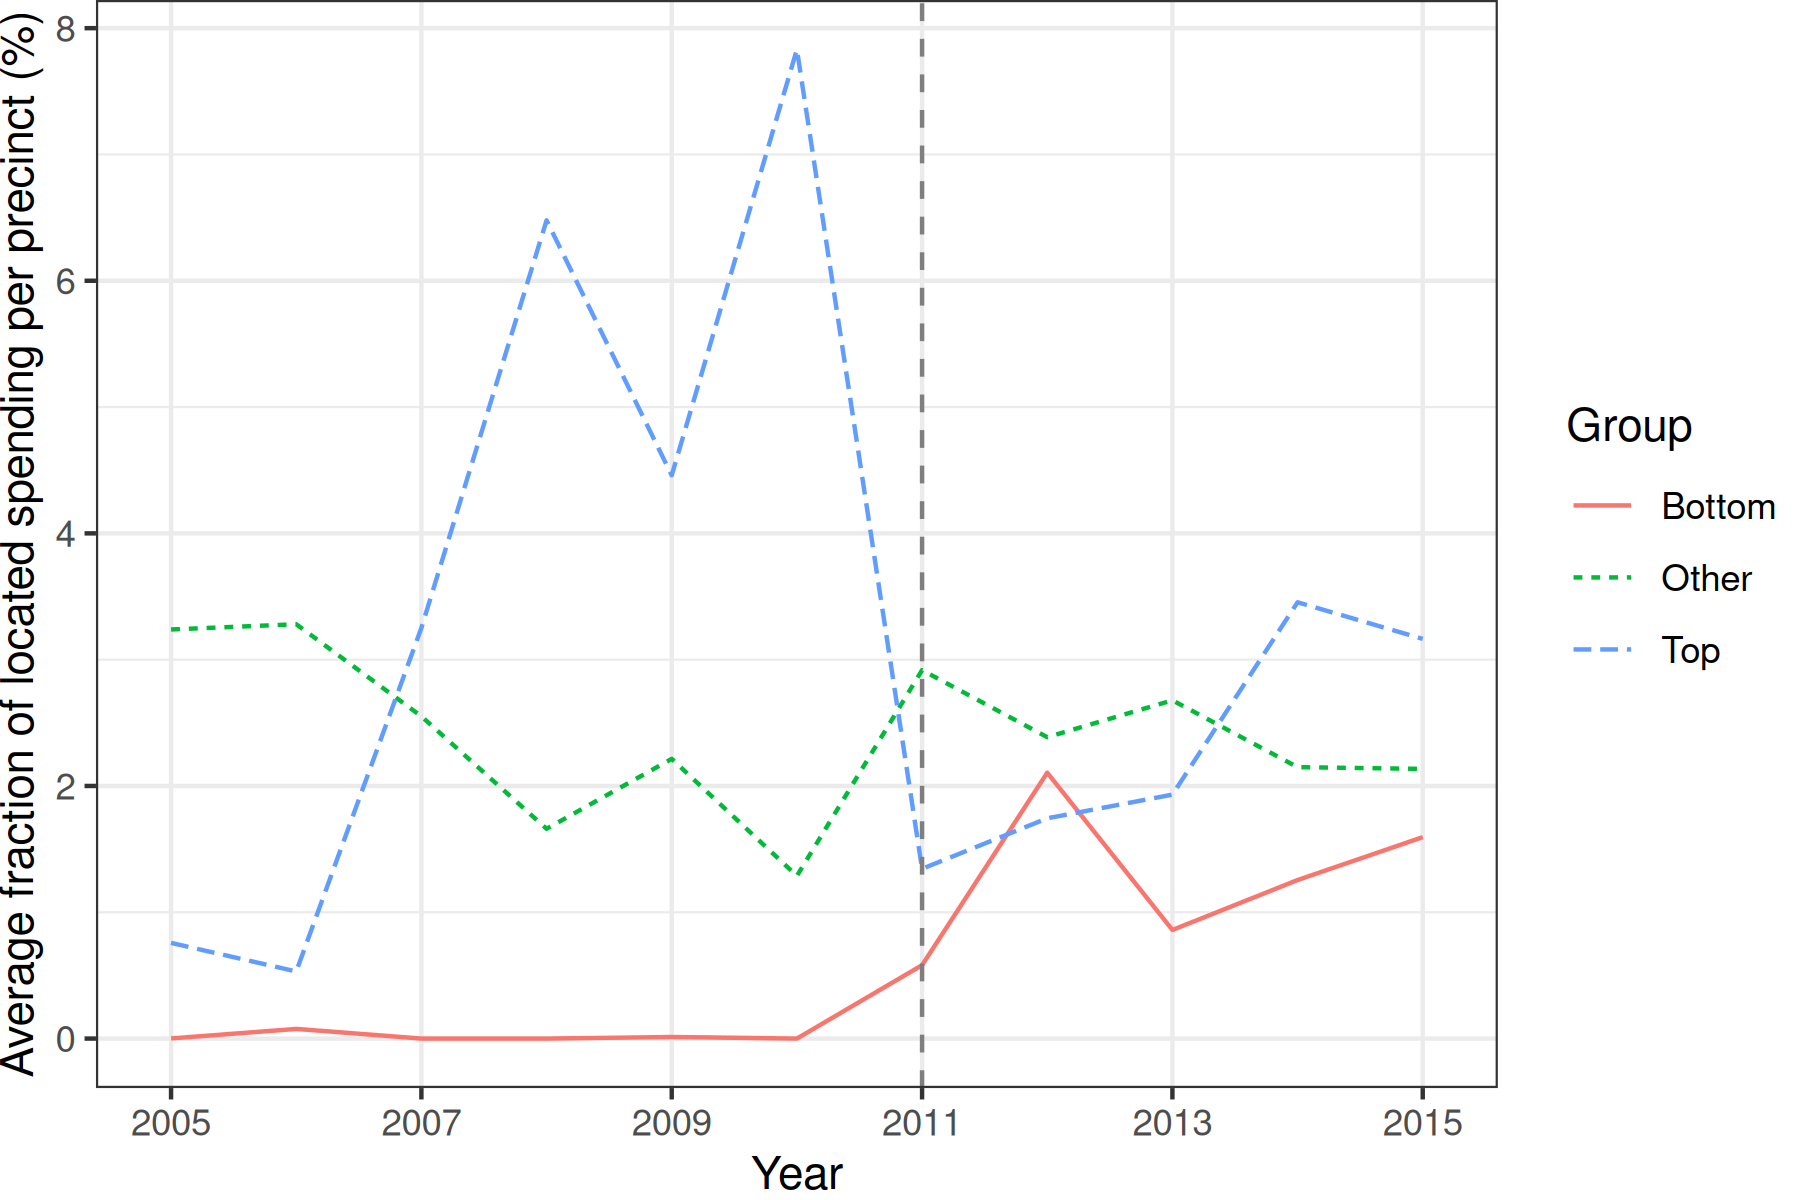
\includegraphics[width=0.8\textwidth]{input/ward_50_contribution_8_precincts_timeline.png}
    \caption{Average Spending per Precinct in the 50th Ward, 2005-2016}
    \label{fig:stone_spending_timeline}
\end{figure}

Finally, we can look at the 50th ward's spending per precinct in the years leading up to and following Stone's defeat in 2011 via a map in Figure~\ref{fig:stone_spending_maps}.
This figure shows a clear shift in spending from the south-western portion of the ward to a roughly even distribution.

\begin{figure}[H]
    \centering
    % First subfigure
    \begin{subfigure}[b]{0.45\textwidth} % [b] aligns at the bottom
    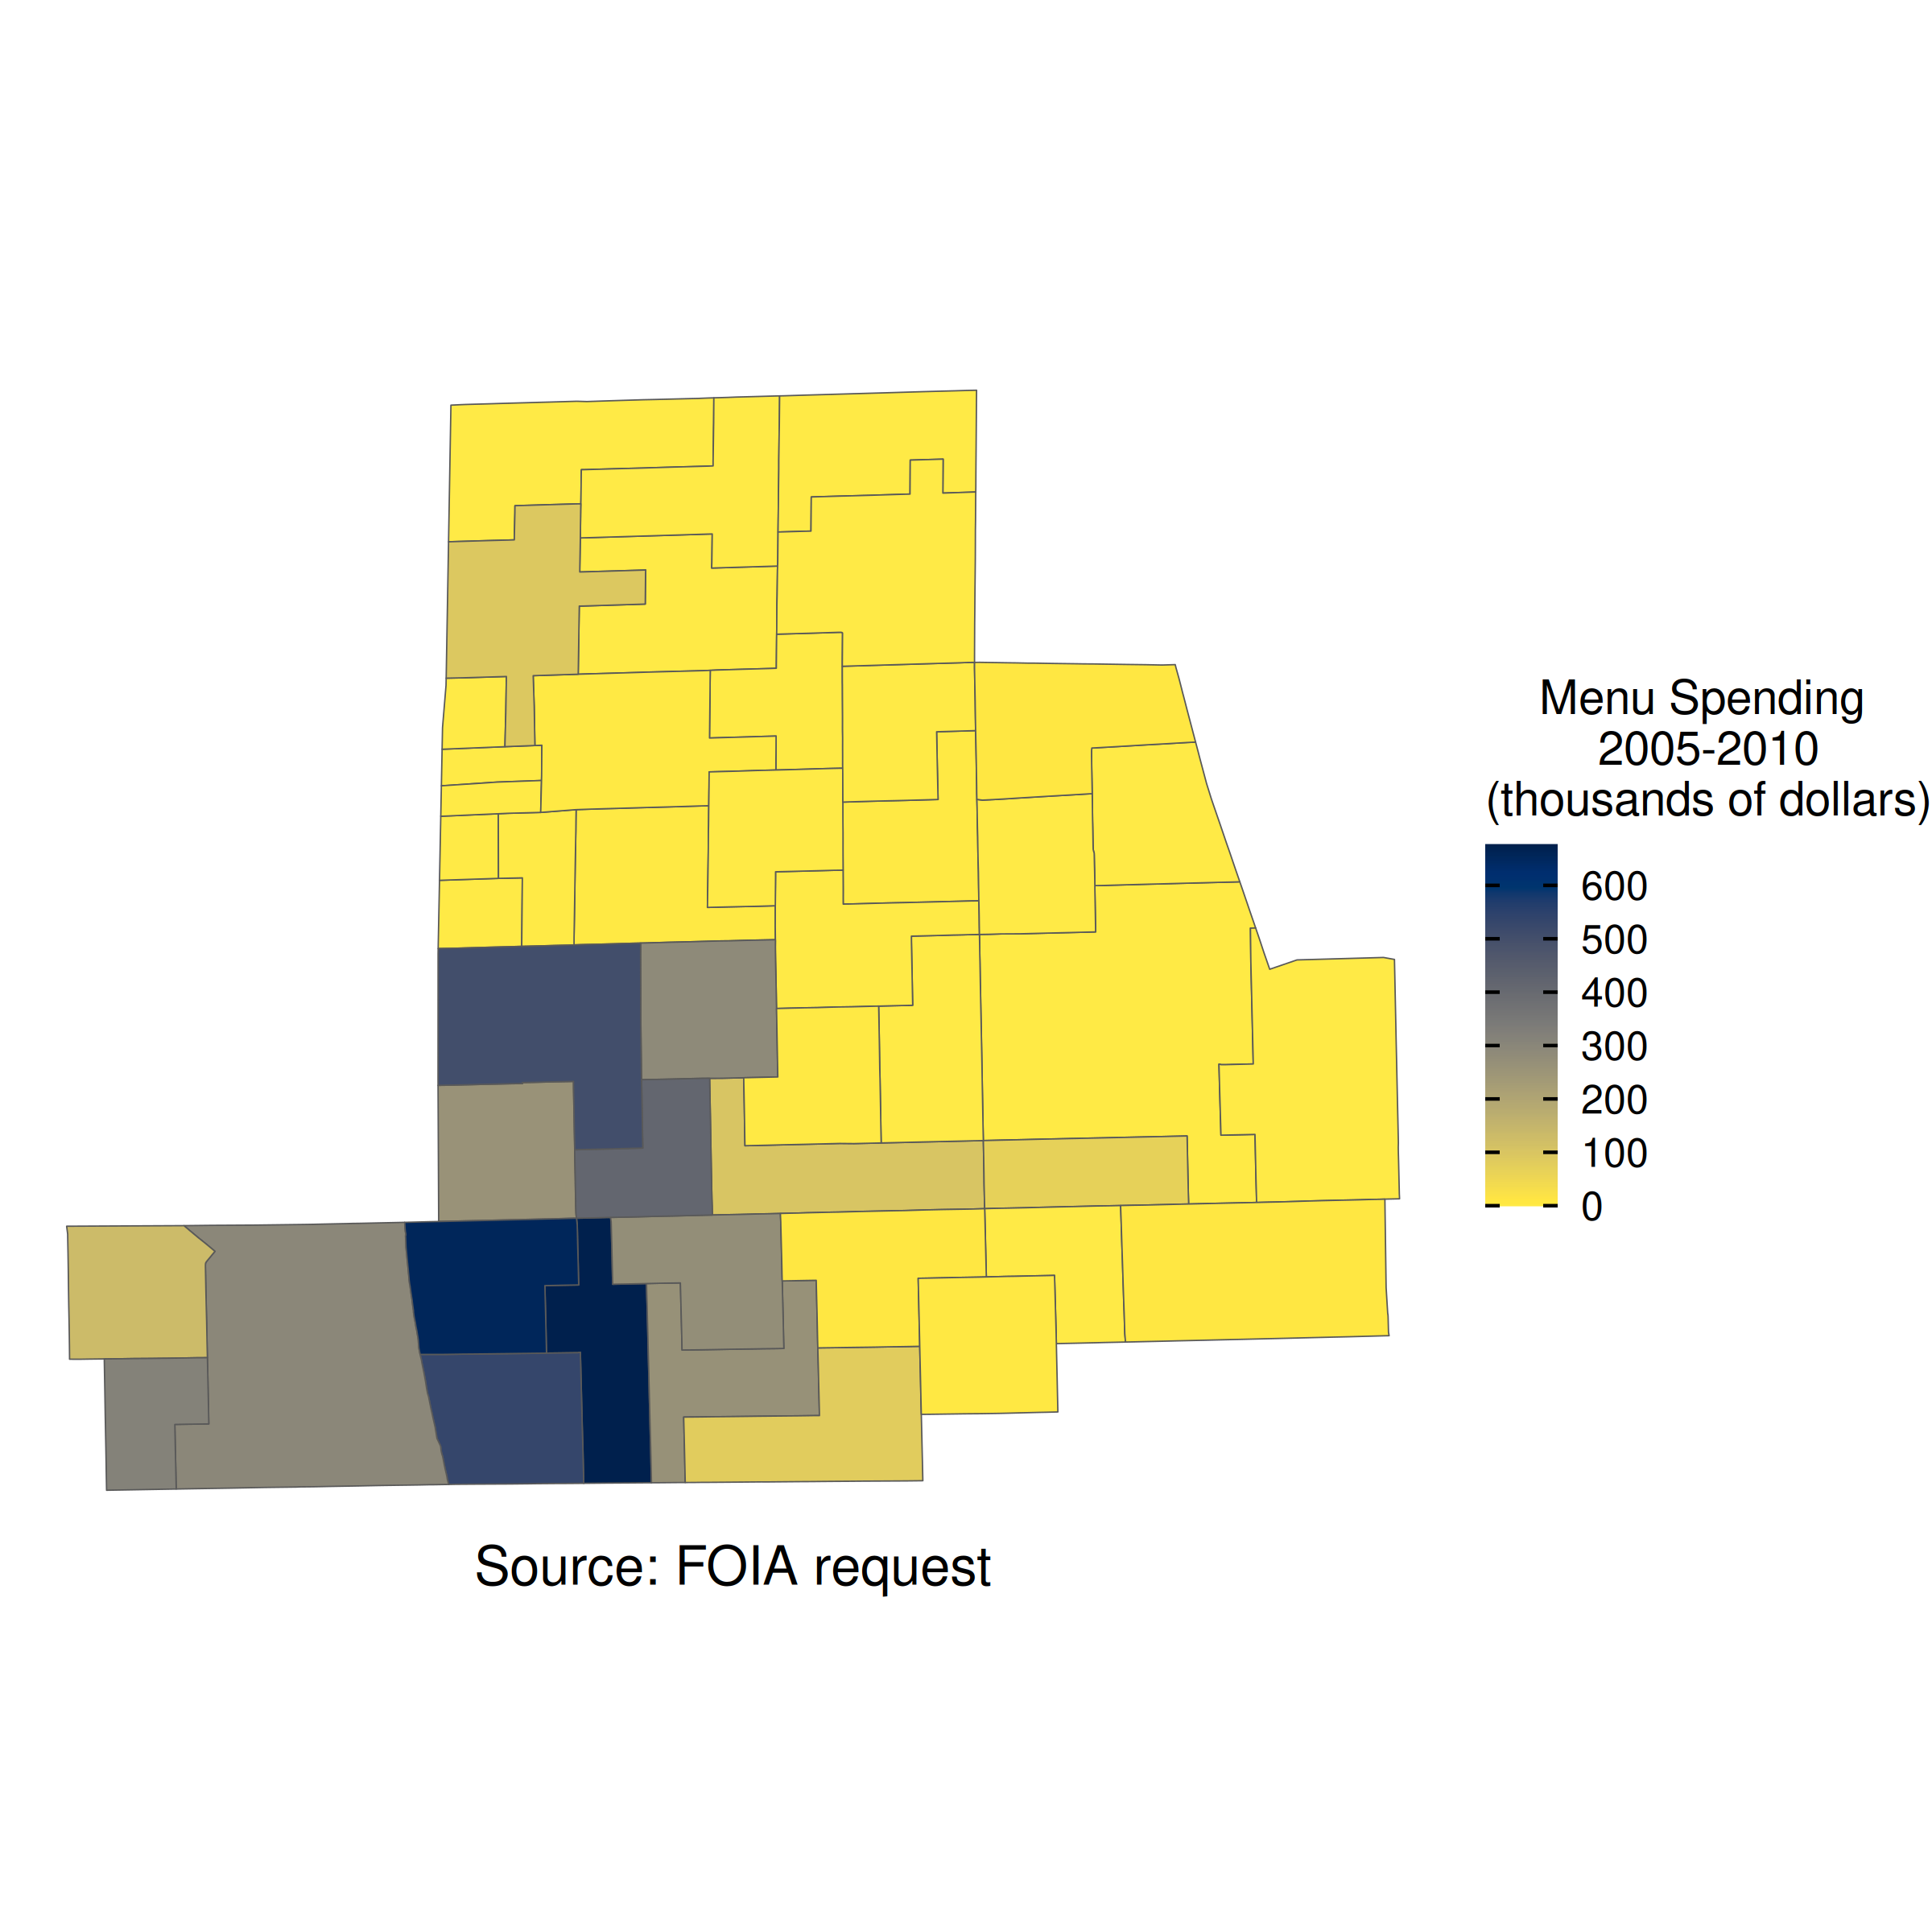
\includegraphics[width=\textwidth]{input/ward_50_menu_map_2005_2010.png}
    \caption{50th Ward Menu Allocation, 2005-2010}
    \end{subfigure}
    \hfill % This adds some space between the two subfigures
    % Second subfigure
    \begin{subfigure}[b]{0.45\textwidth}
    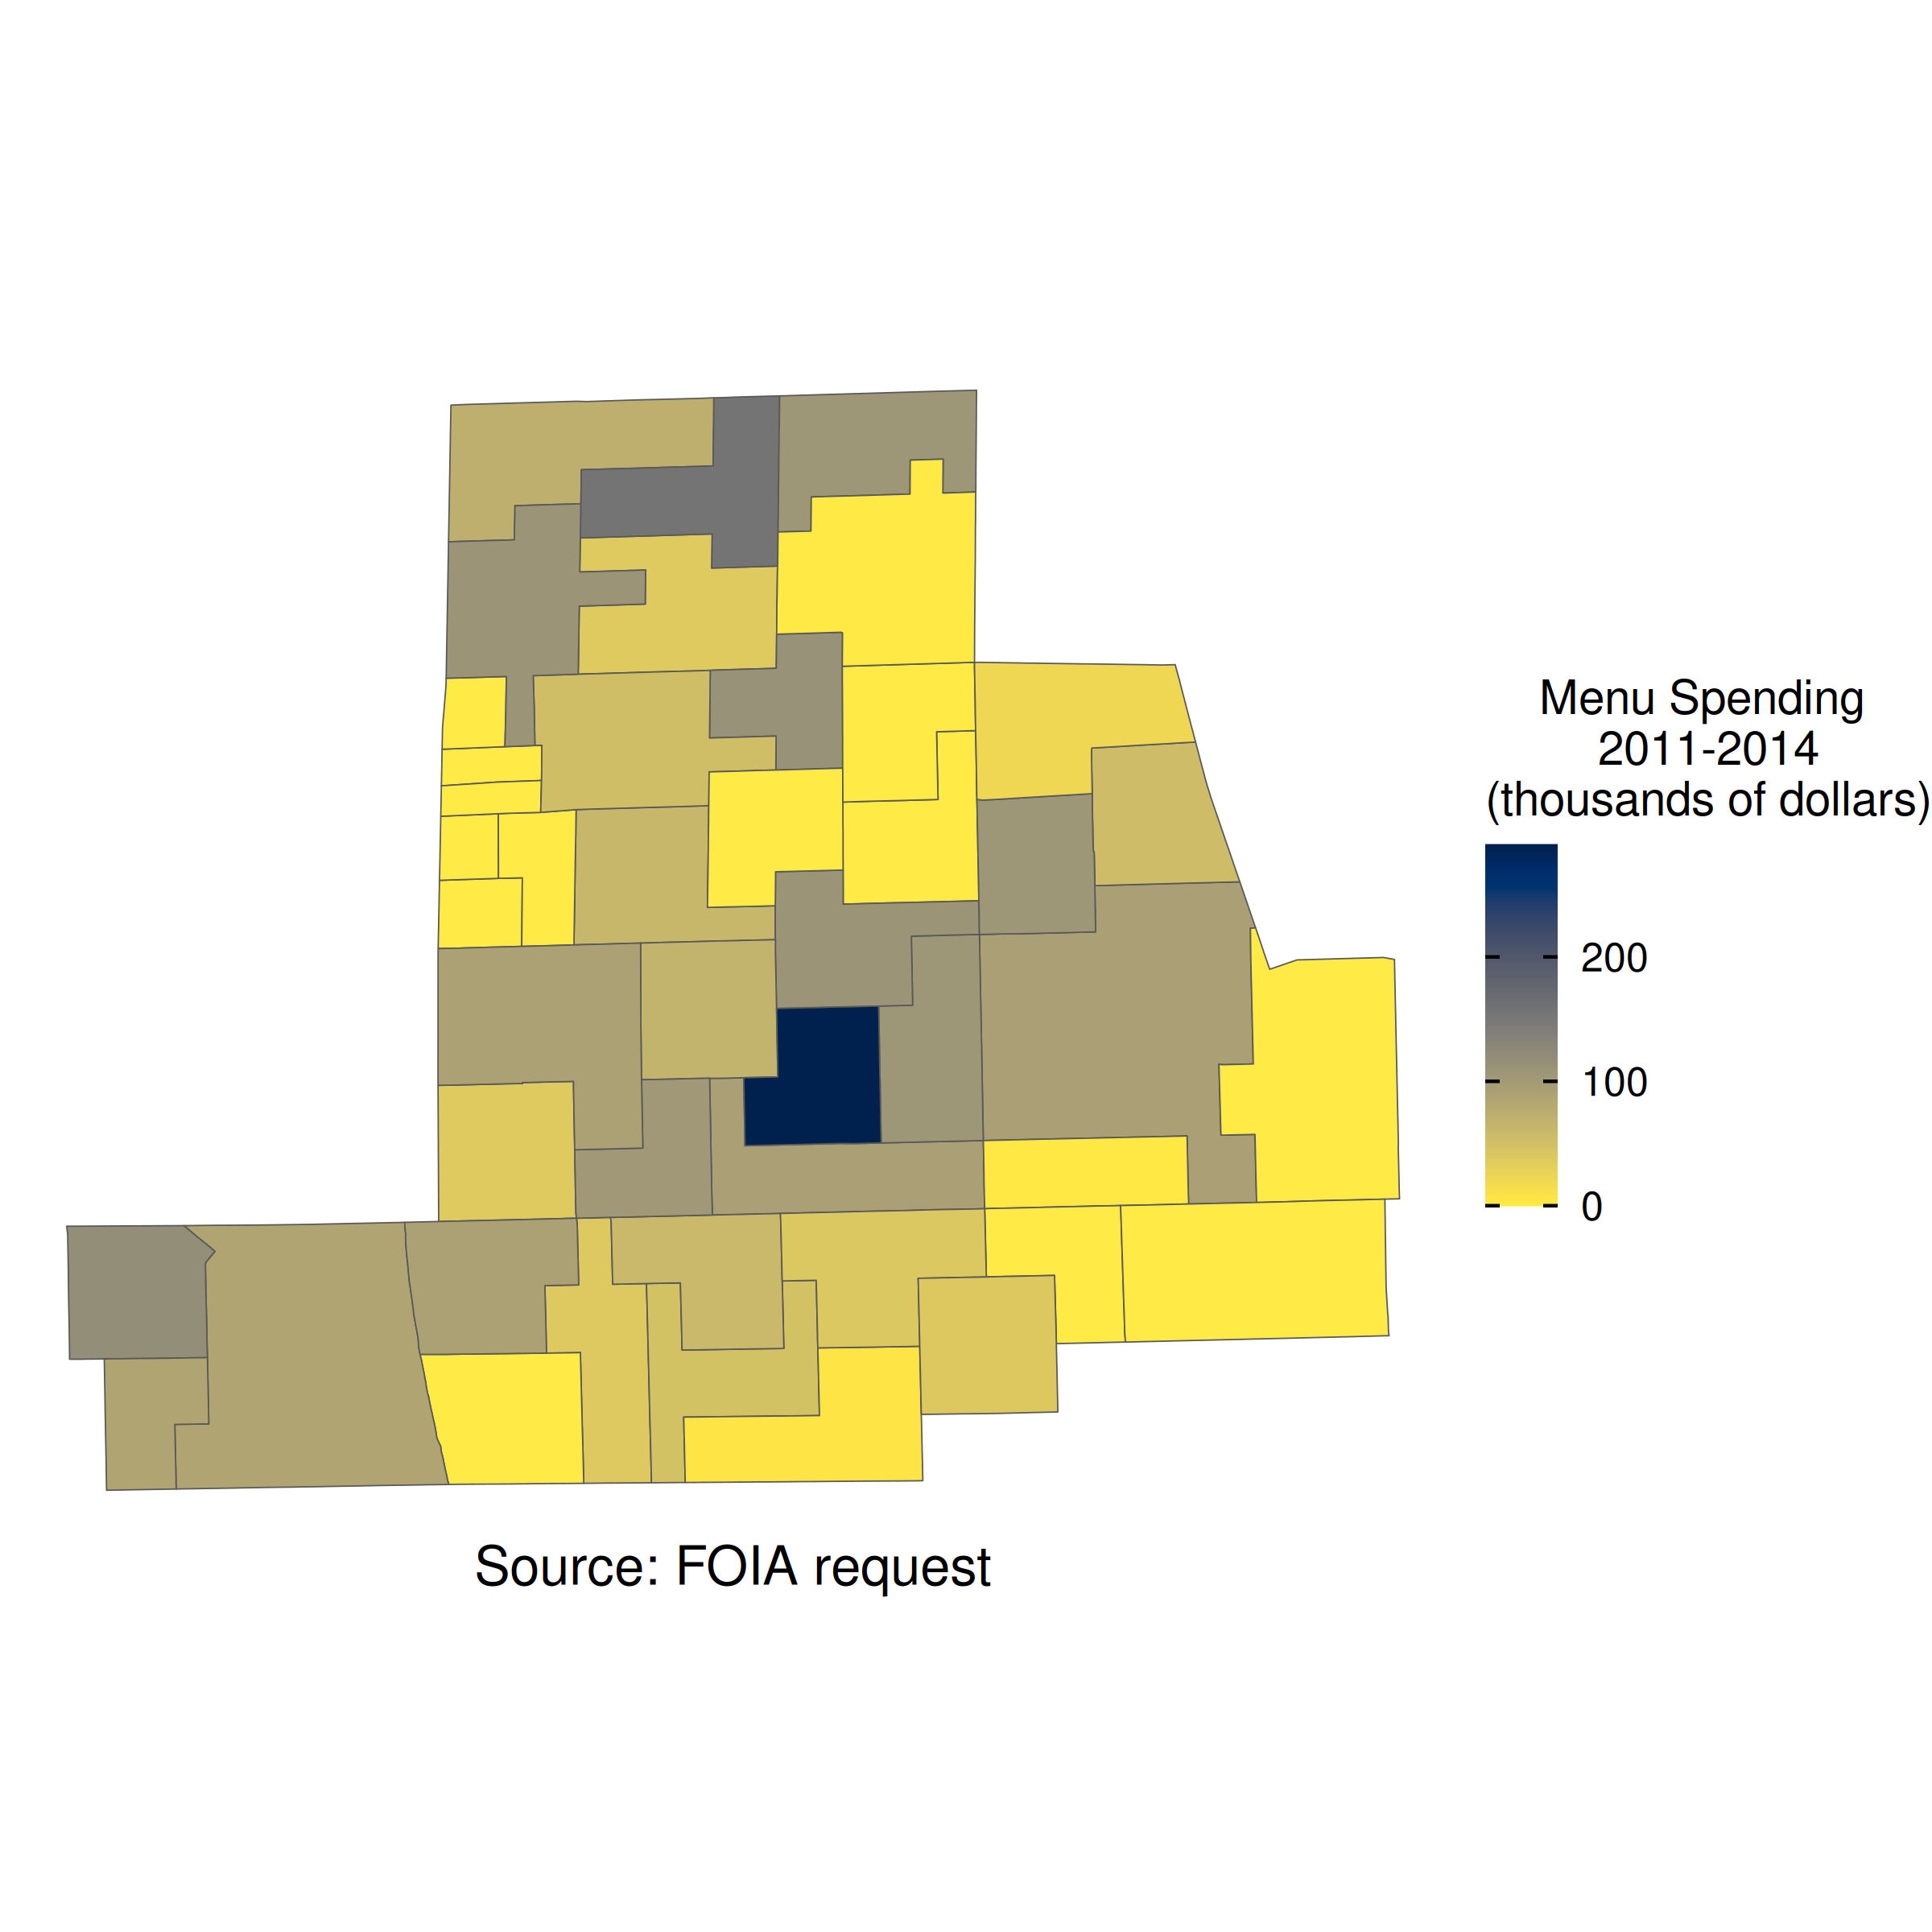
\includegraphics[width=\textwidth]{input/ward_50_menu_map_2011_2014.png}
    \caption{50th Ward Menu Allocation, 2011-2015}
    \end{subfigure}
    \caption{50th Ward Menu Allocation, 2011-2016}
    \label{fig:stone_spending_maps}
\end{figure}


\section{Empirical Framework}\label{sec:empframe}
This section discusses the empirical framework used to analyze the data.
I use the removal of an incumbent from office and the resulting breaking of the incumbent's patronage network to estimate the degree of patronage in the menu program.
To do this, I use a difference-in-differences design to compare the spending trends of supporting or opposing precincts before and after the incumbent leaves office. 
The most standard specification of this design would normally be:

\begin{equation}\label{eq:standard_did}
    Y_{pt} =  \beta T_{pt} + \alpha_{p} + \gamma_{t} + \epsilon_{pt}
\end{equation}

$Y_{pt}$ is the fraction of observed spending in precinct $p$ in year $t$. $T_{pt}$ is a dummy variable equal to 1 if the incumbent alderman was removed from office in year $t$. $\alpha_{p}$ and $\gamma_{t}$ are precinct and year fixed effects respectively. $\epsilon_{pt}$ is the error term.
$\beta$ represents how much spending on an average precinct in the sample changes after an alderman is removed from office.
Thus, in the case of estimating supporting precincts, a negative $\beta$ would indicate that the incumbent alderman was allocating more spending to those that supported them than the following alderman would have chosen.
Under parallel trends and homogenous treatment effects, this represents the causal impact of removing an alderman from office on spending in the precincts contained in the sample.
Yet, this model should not be naively applied with two-way fixed effects due to the recent literature on heterogeneous treatment effects on two-way fixed effects estimators with staggered treatment timing \citep{chaisetwfe} \citep{CALLAWAY2021200}. 
There are a number of ways to address this issue, but I use the heterogeneous-treatment effect robust estimator proposed by \citep{CALLAWAY2021200}\footnote[1]{I do not use a continuous treatment design for reasons specified by \cite{callaway2021_continuous}.
To identify a casual response using a continuous treatment requires that low-dosage groups (ie, middling supporting precincts) would have the same response had they chosen a high level of support instead.
This is in fact directly at odds with the \cite{dixit_londregan1996} model's implication that for machine politics to exist, the politician must be able to distribute goods more efficiently to supporters than non-supporters.
Therefore, using a continuous treatment design would be effectively assuming away the very phenomenon the design is estimating.}.


This paper estimates four variations of equation \ref{eq:standard_did}. 
The first two rely on a close-election assumption to justify the parallel trends assumption. 
This assumption means incumbent aldermen who win by a small margin have similar spending trends to those who lose by a small margin.
This study defines a close margin as 10\% or less; this corresponds to approximately 1,200 votes.
This assumption effectively means that incumbent aldermen who barely win allocate funds similarly to those who barely lose in the run-up to the election.
I then examine two sets of precincts. 
The first set of precincts is the top quintile (8) precincts by vote margin for each ward in the 2015 or 2019 election, whichever is appropriate to the treatment group. 
The second set of precincts is the bottom quintile precincts by vote margin for each ward in the 2015 or 2019 election, whichever is appropriate to the treatment group.
I use the years 2012 through 2022 to estimate this model due to the 2011 redistricting complicating the use of 2005-2011 data. 

The third and fourth variations rely on a simultaneous set of indictments of aldermen in 2019, causing three aldermen to either be ineligible for reelection or to retire. 
These aldermen were Daniel Solis, Ricardo Munoz, and Willie Cochran. 
Daniel Solis left office after being caught for corruption by the FBI and wearing a wire to record Alderman Ed Burke, who was indicted in 2019 but not removed from office until 2023.
Ricardo Munoz retired after reporters discovered he spent PAC money on personal expenses.
Willie Cochran retired after pleading guilty to wire fraud and misusing campaign funds for gambling and personal expenses.
I compare this group to a set of 10 control aldermen who were not indicted, have been in office for at least 10 years, and won reelection in 2019 in the general election, indicating they were not in a competitive election. 
To measure whether or not a precinct supported an alderman, I use the total number of campaign contributions donated to the aldermen from the precinct in the 2015 and 2019 elections.
I do this because many ``entrenched'' aldermen have not faced a competitive election in decades, so net votes are not a good measure of support.
Despite this, all aldermen still accept campaign contributions even when there is no challenger, so I use this to measure support.
In this case, I expect the trends for the indicted and control aldermen will be the same, as they are all not in competitive elections, and thus, their spending preferences should be stable over time.
Furthermore, the unexpected timing of indictments within the election would hopefully preclude any anticipatory behavior.
In both cases, I cluster standard errors at the ward level.
\section{Results}\label{sec:results}


I compute the dynamic aggregation of the average treatment effect on the treated group for the least and most supporting precincts and display the results in Table~\ref{tab:att_comparison_combined}.
Also shown are the estimate's standard errors, confidence intervals, and Wald-test p-values for the pre-test of the parallel trends assumption.
Both estimated ATTs are not statistically significant for the close election design.
Furthermore, the least supporting precinct's ATT is not especially economically significant. 
Half a percent of the menu program's budget is roughly \$7,500. 
That is not even enough to afford two speed humps.
Additionally concerning are the extremely low p-values for the pre-trends test.
This test indicates that the close election design likely does not guarantee that parallel trends hold.
This failure may be because factors influencing the trend of infrastructure spending and needs correlate with the election outcome.
Alternatively, it could be because the margin chosen is too large to ensure that the two groups are similar.
The results of the competitive elections design is susceptible to the number of precincts included, often changing the sign of both estimated ATTs.
Note that the treatment effect for the least supporting precincts is over five times larger than the treatment effect estimated in the competitive election design.
Table~\ref{tab:att_comparison_combined} shows a much larger Wald-test p-value for the pre-trends test.
These values indicate that perhaps the indictment design's assumption is more believable than the close election design's assumption.
However, I also see that the most supporting precinct's treatment effect, while statistically significant, is similar in magnitude to the treatment effect of the competitive election design.

\begin{table}[H]
    \centering
    \caption{Comparison of average treatment effects}
    \label{tab:att_comparison_combined}
    \begin{tabular}{lcc|cc}
    \hline
     & \multicolumn{2}{c|}{Competitive Election} & \multicolumn{2}{c}{Indictment} \\
     & Opposing ATT & Supporting ATT & Opposing ATT & Supporting ATT \\
    \hline
    ATT & 0.50 (0.45) & -1.51 (1.12) & 2.59 (0.78) & -1.15 (0.32) \\
    95\% Conf. Int. & (-0.38, 1.39) & (-3.71, 0.68) & (1.06, 4.11) & (-1.77, -0.52) \\
    Pre-Trends P-value & 0.005  & 0.076 & 0.199 & 0.174 \\
    Observations & 1680 & 1680 & 1144 & 1144 \\
    \hline
    \end{tabular}
\end{table}

Figure~\ref{fig:ATT_over_time} depicts how all all of the four design's estimated ATTs vary over time.
All of the designs except for Panel~\ref{fig:ATT_over_time:corruption_top}  pass a placebo test in last several years before the first treatment.
Panel~\ref{fig:ATT_over_time:corruption_top} shows evidence of anticipation in the year before the first treatment, as the 2019 estimate is significantly smaller than the other estimates.
As inferred from the standard errors in Table~\ref{tab:att_comparison_combined}, the estimated effect over time is noisy for all four designs.
The large noise is likely because even a benevolent social planner will not allocate infrastructure spending using a highly auto-correlated spending rule.
A road, once paved, does not need to be repaved for approximately 20 years according to CDOT's life cycle analysis \citep{OIGaudit}.
There is a limit to how much spending can be preferentially allocated to a precinct before that alderman runs into harshly diminishing returns.
Despite this, Panels~\ref{fig:ATT_over_time:corruption_bottom} and~\ref{fig:ATT_over_time:corruption_top} both show statistically significant effects post-treatment.
The standard errors, while large, are much smaller for these panels, and the mean estimate is much more stable.
This holds for the most supporting precincts as well, albeit in reverse.
Thus, as the incumbent alderman leaves office, they allocate more spending to their most supporting precincts than their least keeping precincts.
These results must be taken with a grain of salt due to the high standard errors and the likely pre-trends violation.

\begin{figure}[H]
    \centering
    \caption{ATT over time for the four designs}
    \label{fig:ATT_over_time}

    % First row
    \begin{subfigure}{.48\linewidth}
        \centering
        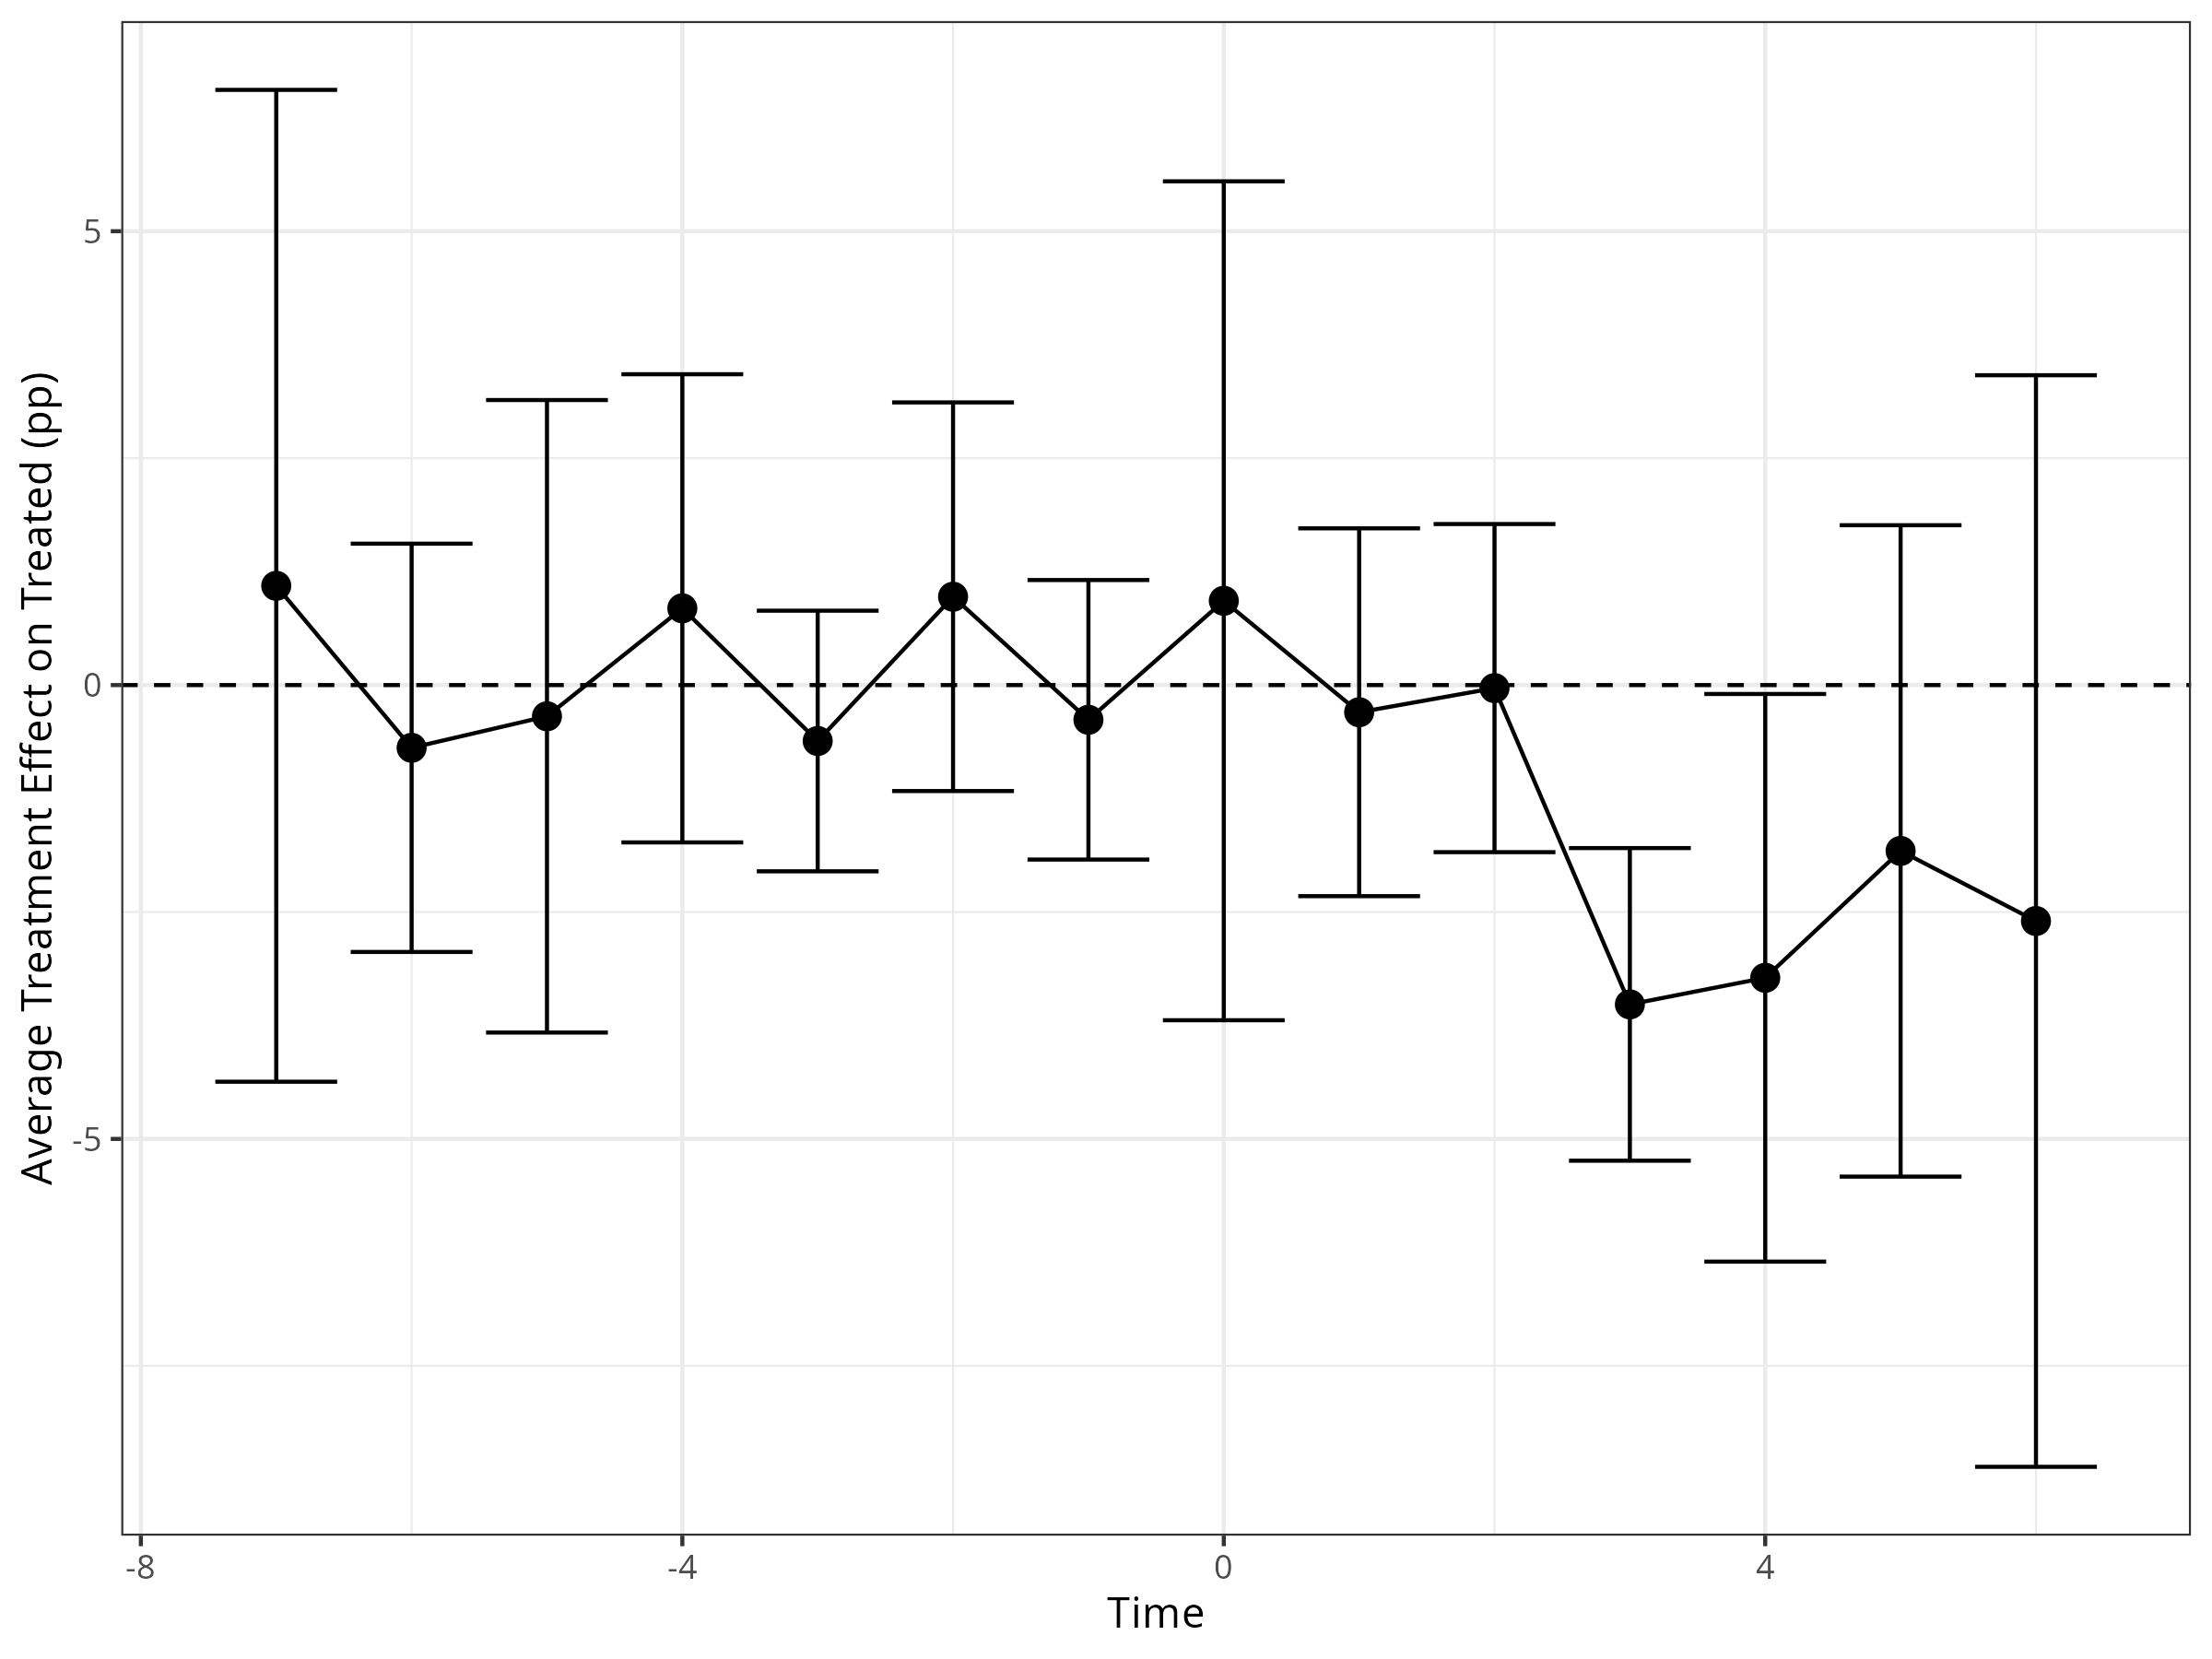
\includegraphics[width=\linewidth]{input/close_elections_8_top_over_time.png}
        \caption{Close Election: most supporting precincts}
        \label{fig:ATT_over_time:close_election_top}
    \end{subfigure}\hfill
    \begin{subfigure}{.48\linewidth}
        \centering
        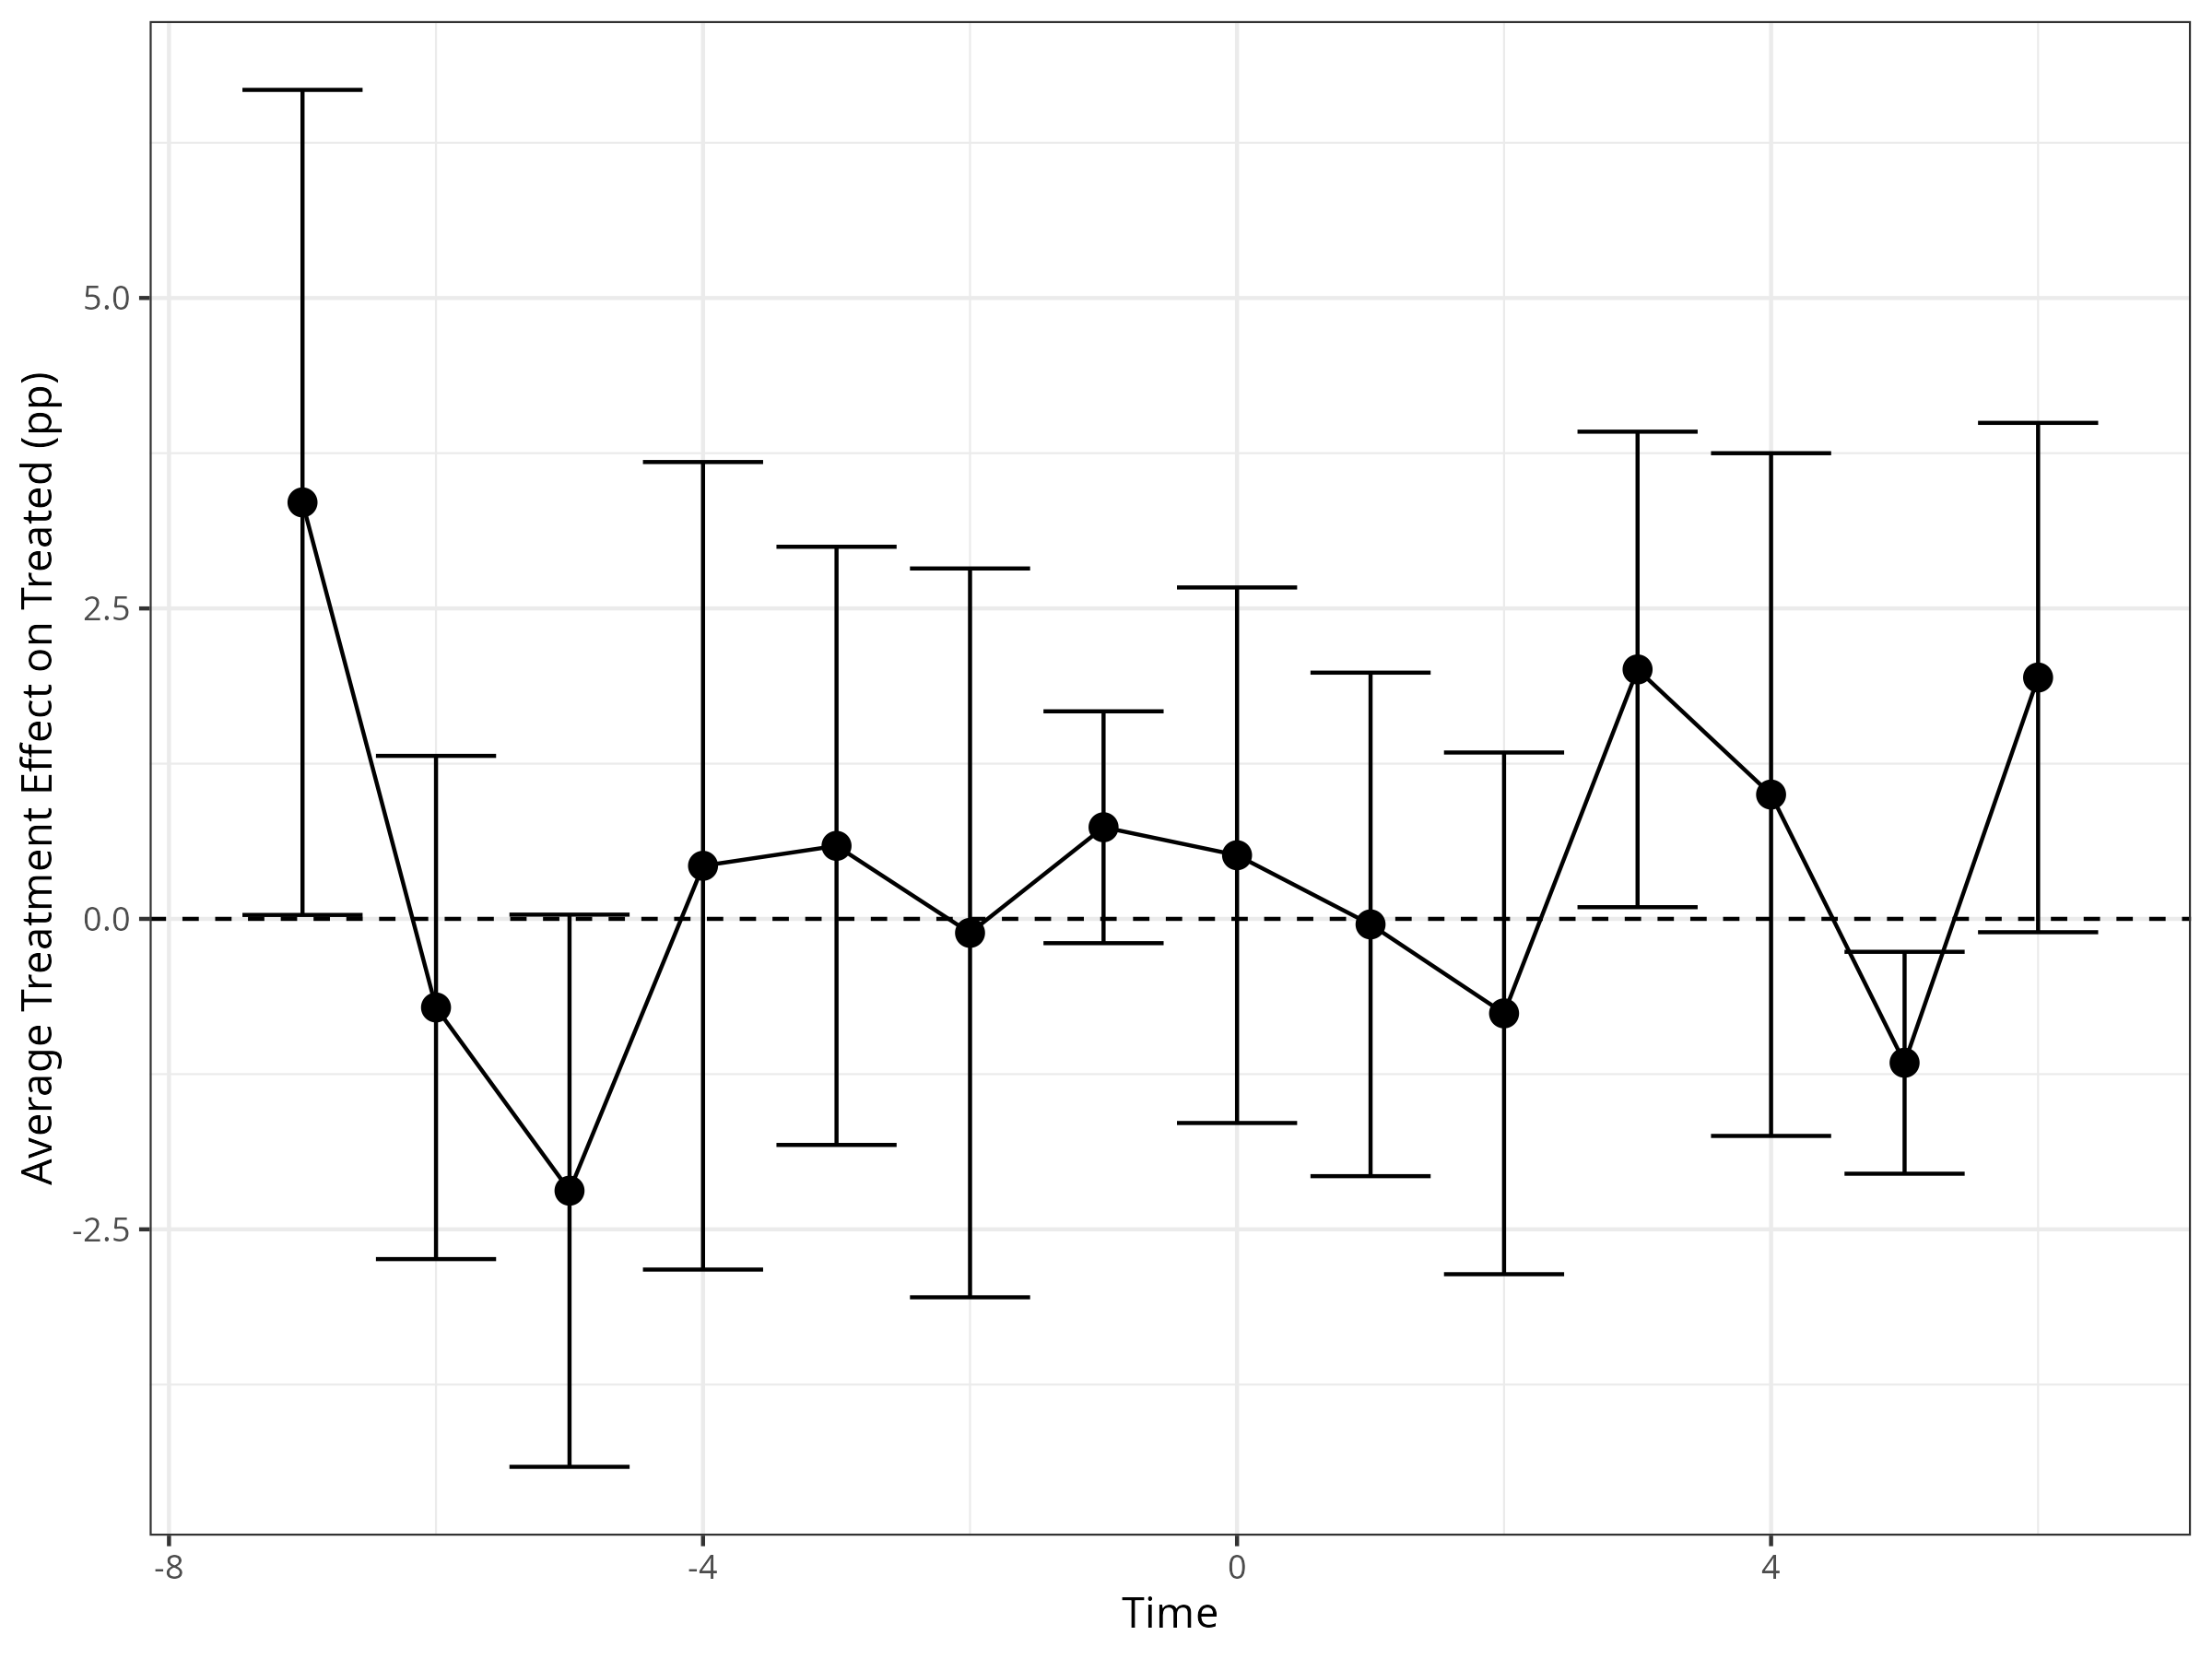
\includegraphics[width=\linewidth]{input/close_elections_8_bottom_over_time.png}
        \caption{Close Election: least supporting precincts}
        \label{fig:ATT_over_time:close_election_bottom}
    \end{subfigure}

    % Second row
    \begin{subfigure}{.48\linewidth}
        \centering
        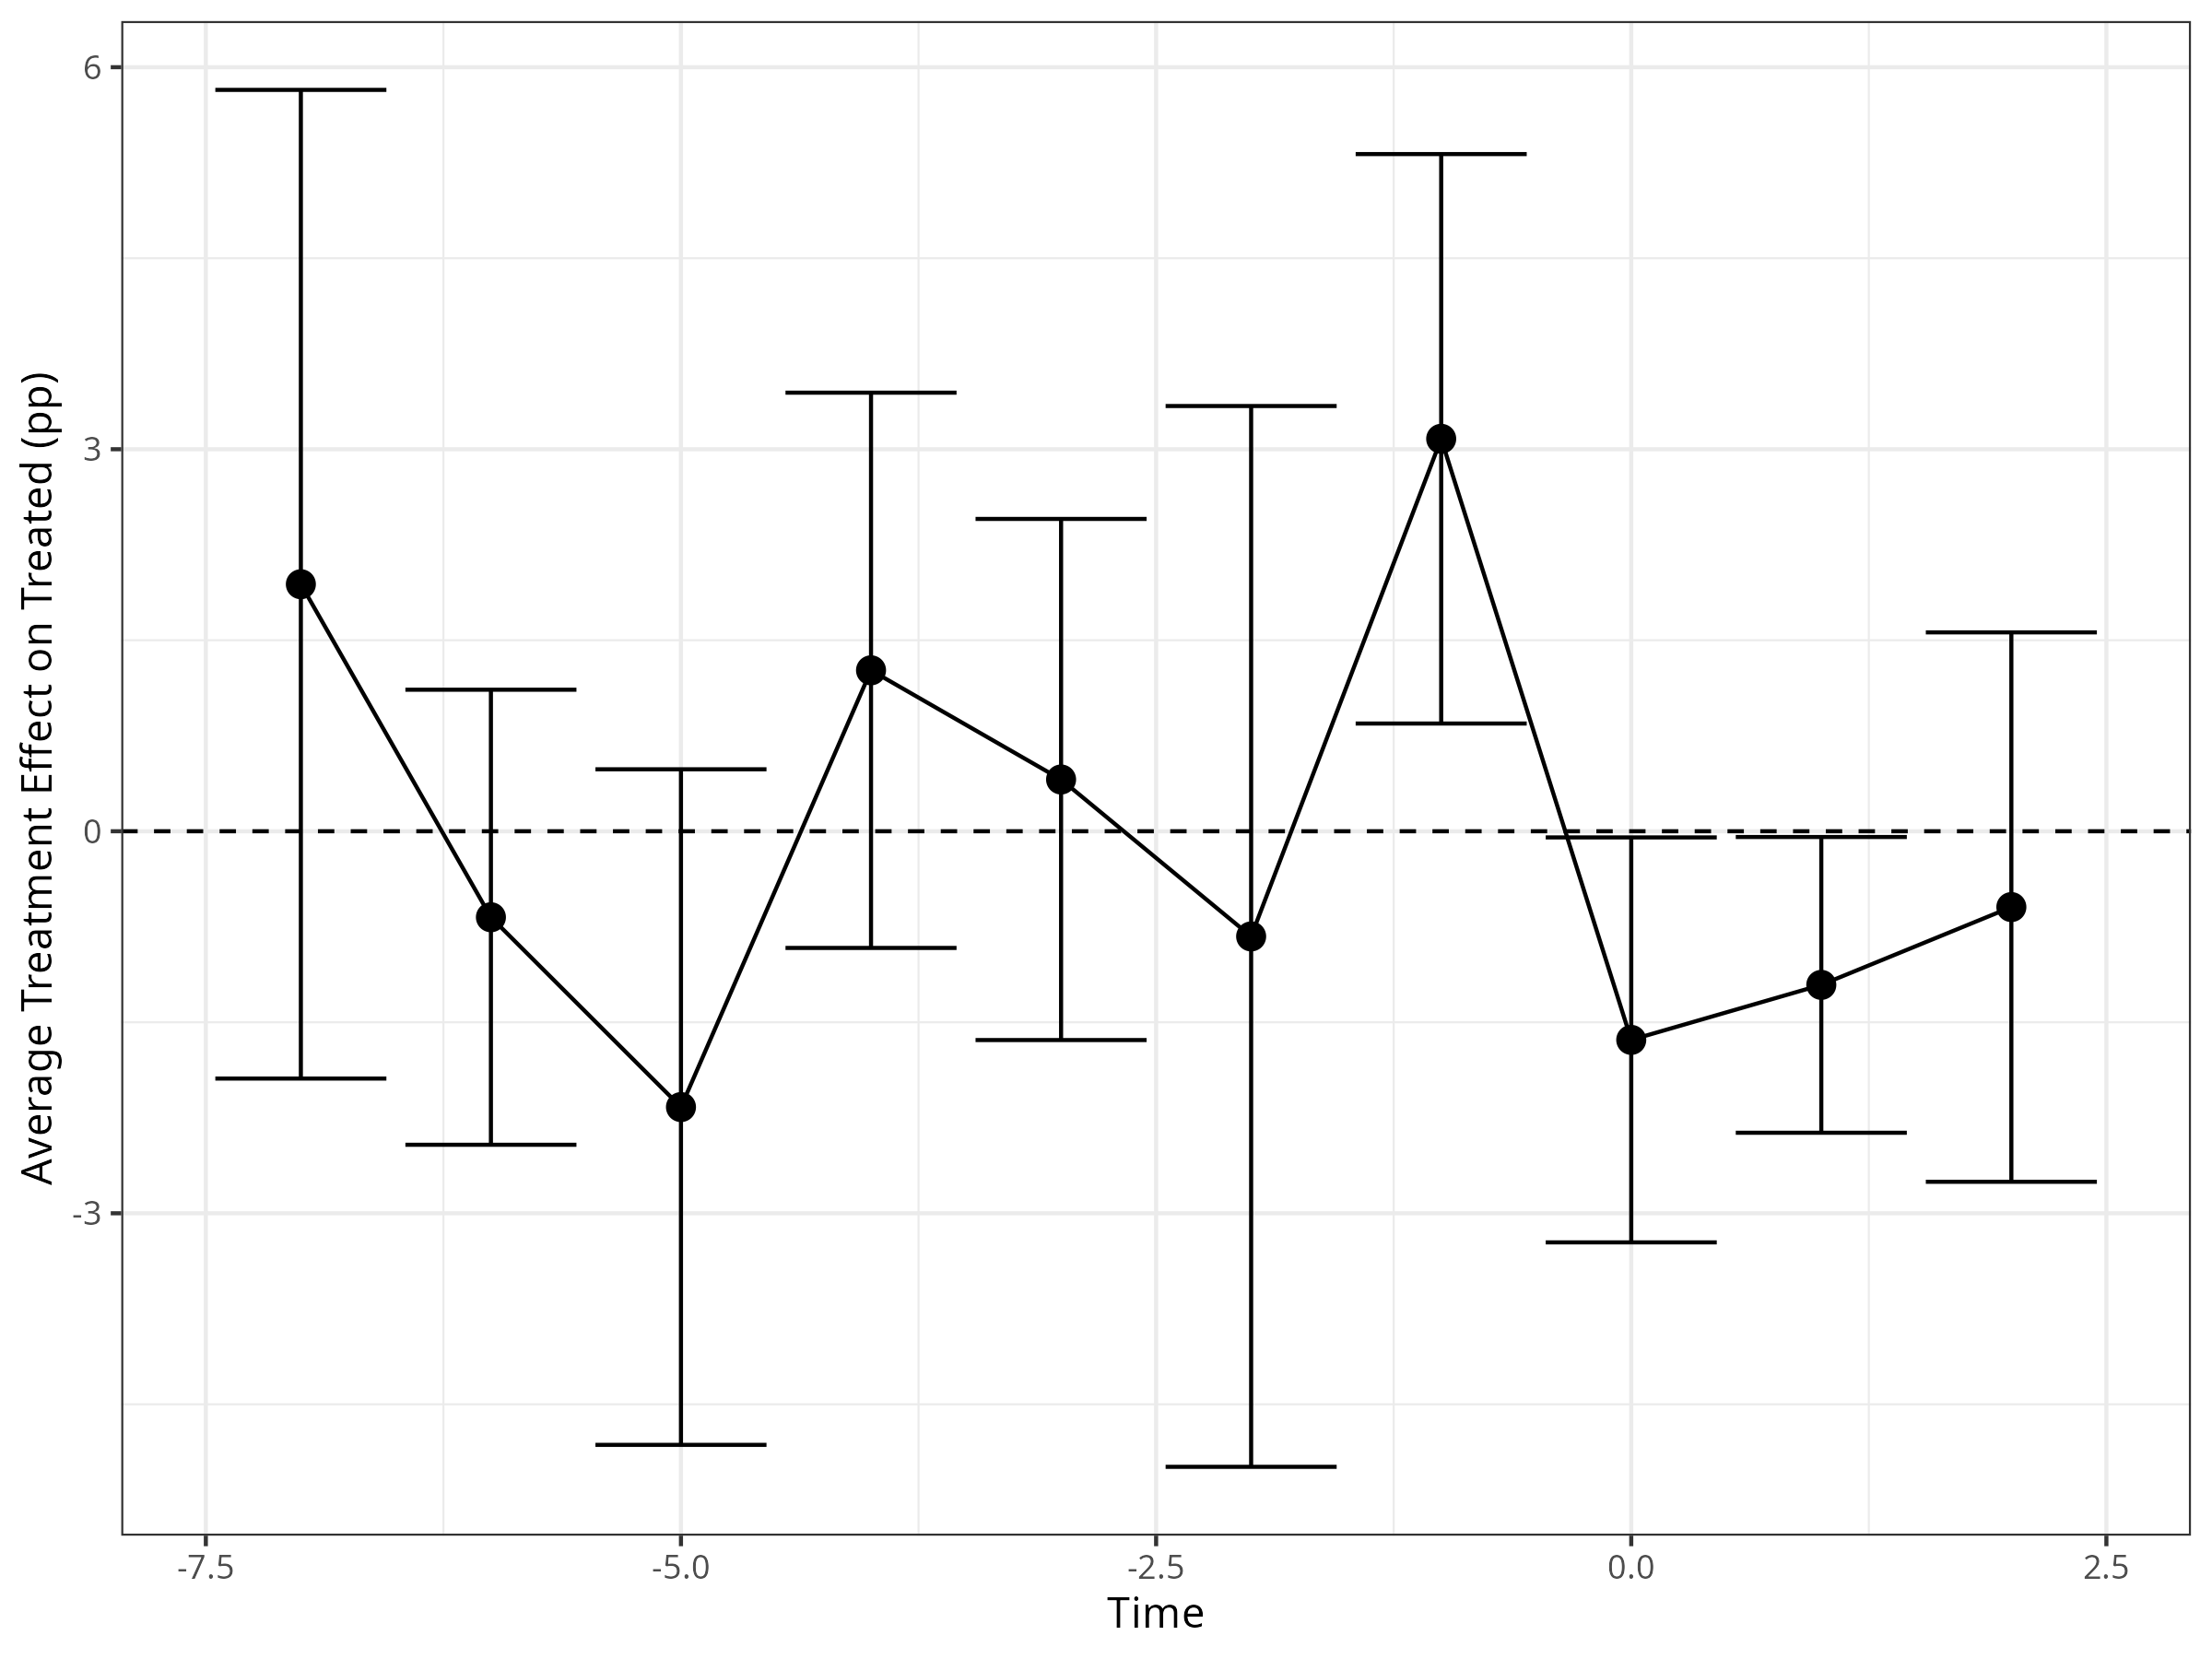
\includegraphics[width=\linewidth]{input/corrupt_8_top_over_time.png}
        \caption{Corruption: most supporting precincts}
        \label{fig:ATT_over_time:corruption_bottom}
    \end{subfigure}\hfill
    \begin{subfigure}{.48\linewidth}
        \centering
        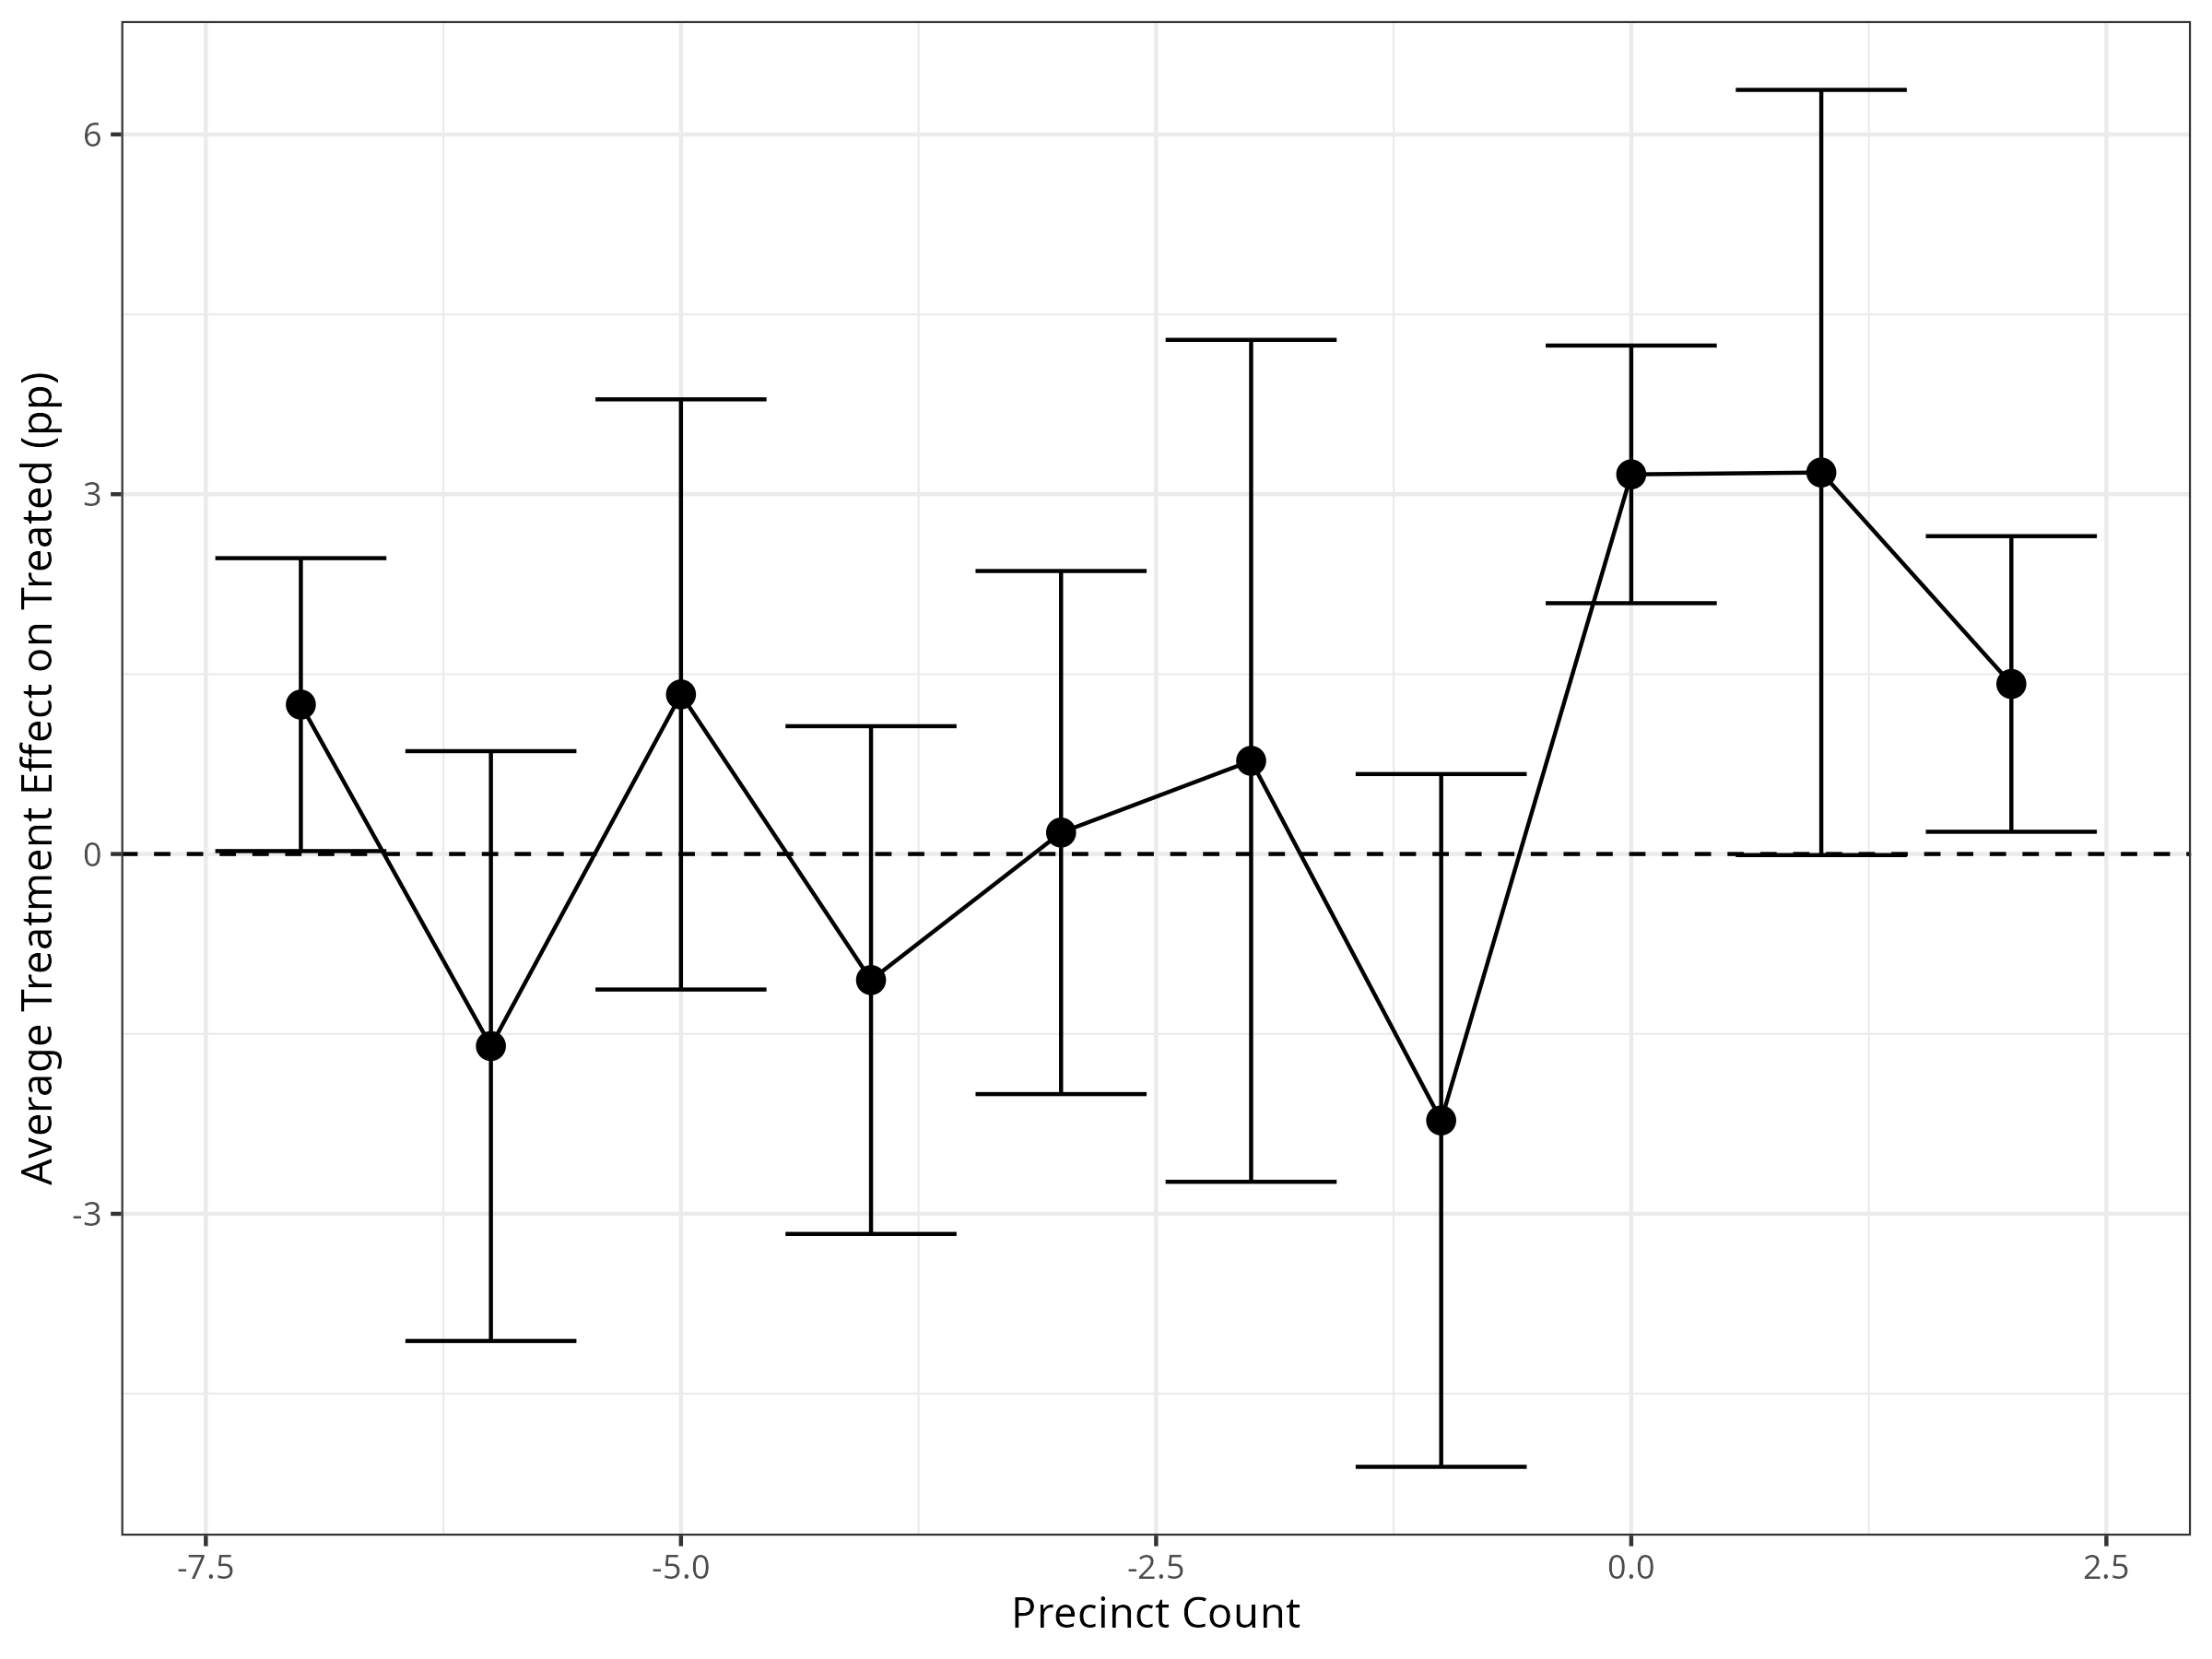
\includegraphics[width=\linewidth]{input/corrupt_8_bottom_over_time.png}
        \caption{Corruption: least supporting precincts}
        \label{fig:ATT_over_time:corruption_top}
    \end{subfigure}
\end{figure}

Lastly, the high standard errors beg the question of how stable the estimates are to the specification used.
The specifications above use the top or bottom supporting quintile, which is 8 precincts as the 2012-2022 period has an average of 41.38 precincts. 
What happens when this number is varied?
Figure~\ref{fig:ATT_across_precincts} shows the estimated ATTs for different numbers of precincts. 
The answer is that the estimates for the least supporting precincts are relatively stable in magnitude, but is only statistically significant for precincts 3-8.
Most supporting precincts seem much more stable, as they are statistically significant for precincts 8-12. 

\begin{figure}[H]
    \centering
    \caption{ATT across number of precincts used}
    \label{fig:ATT_across_precincts}

    % First row
    \begin{subfigure}{.48\linewidth}
        \centering
        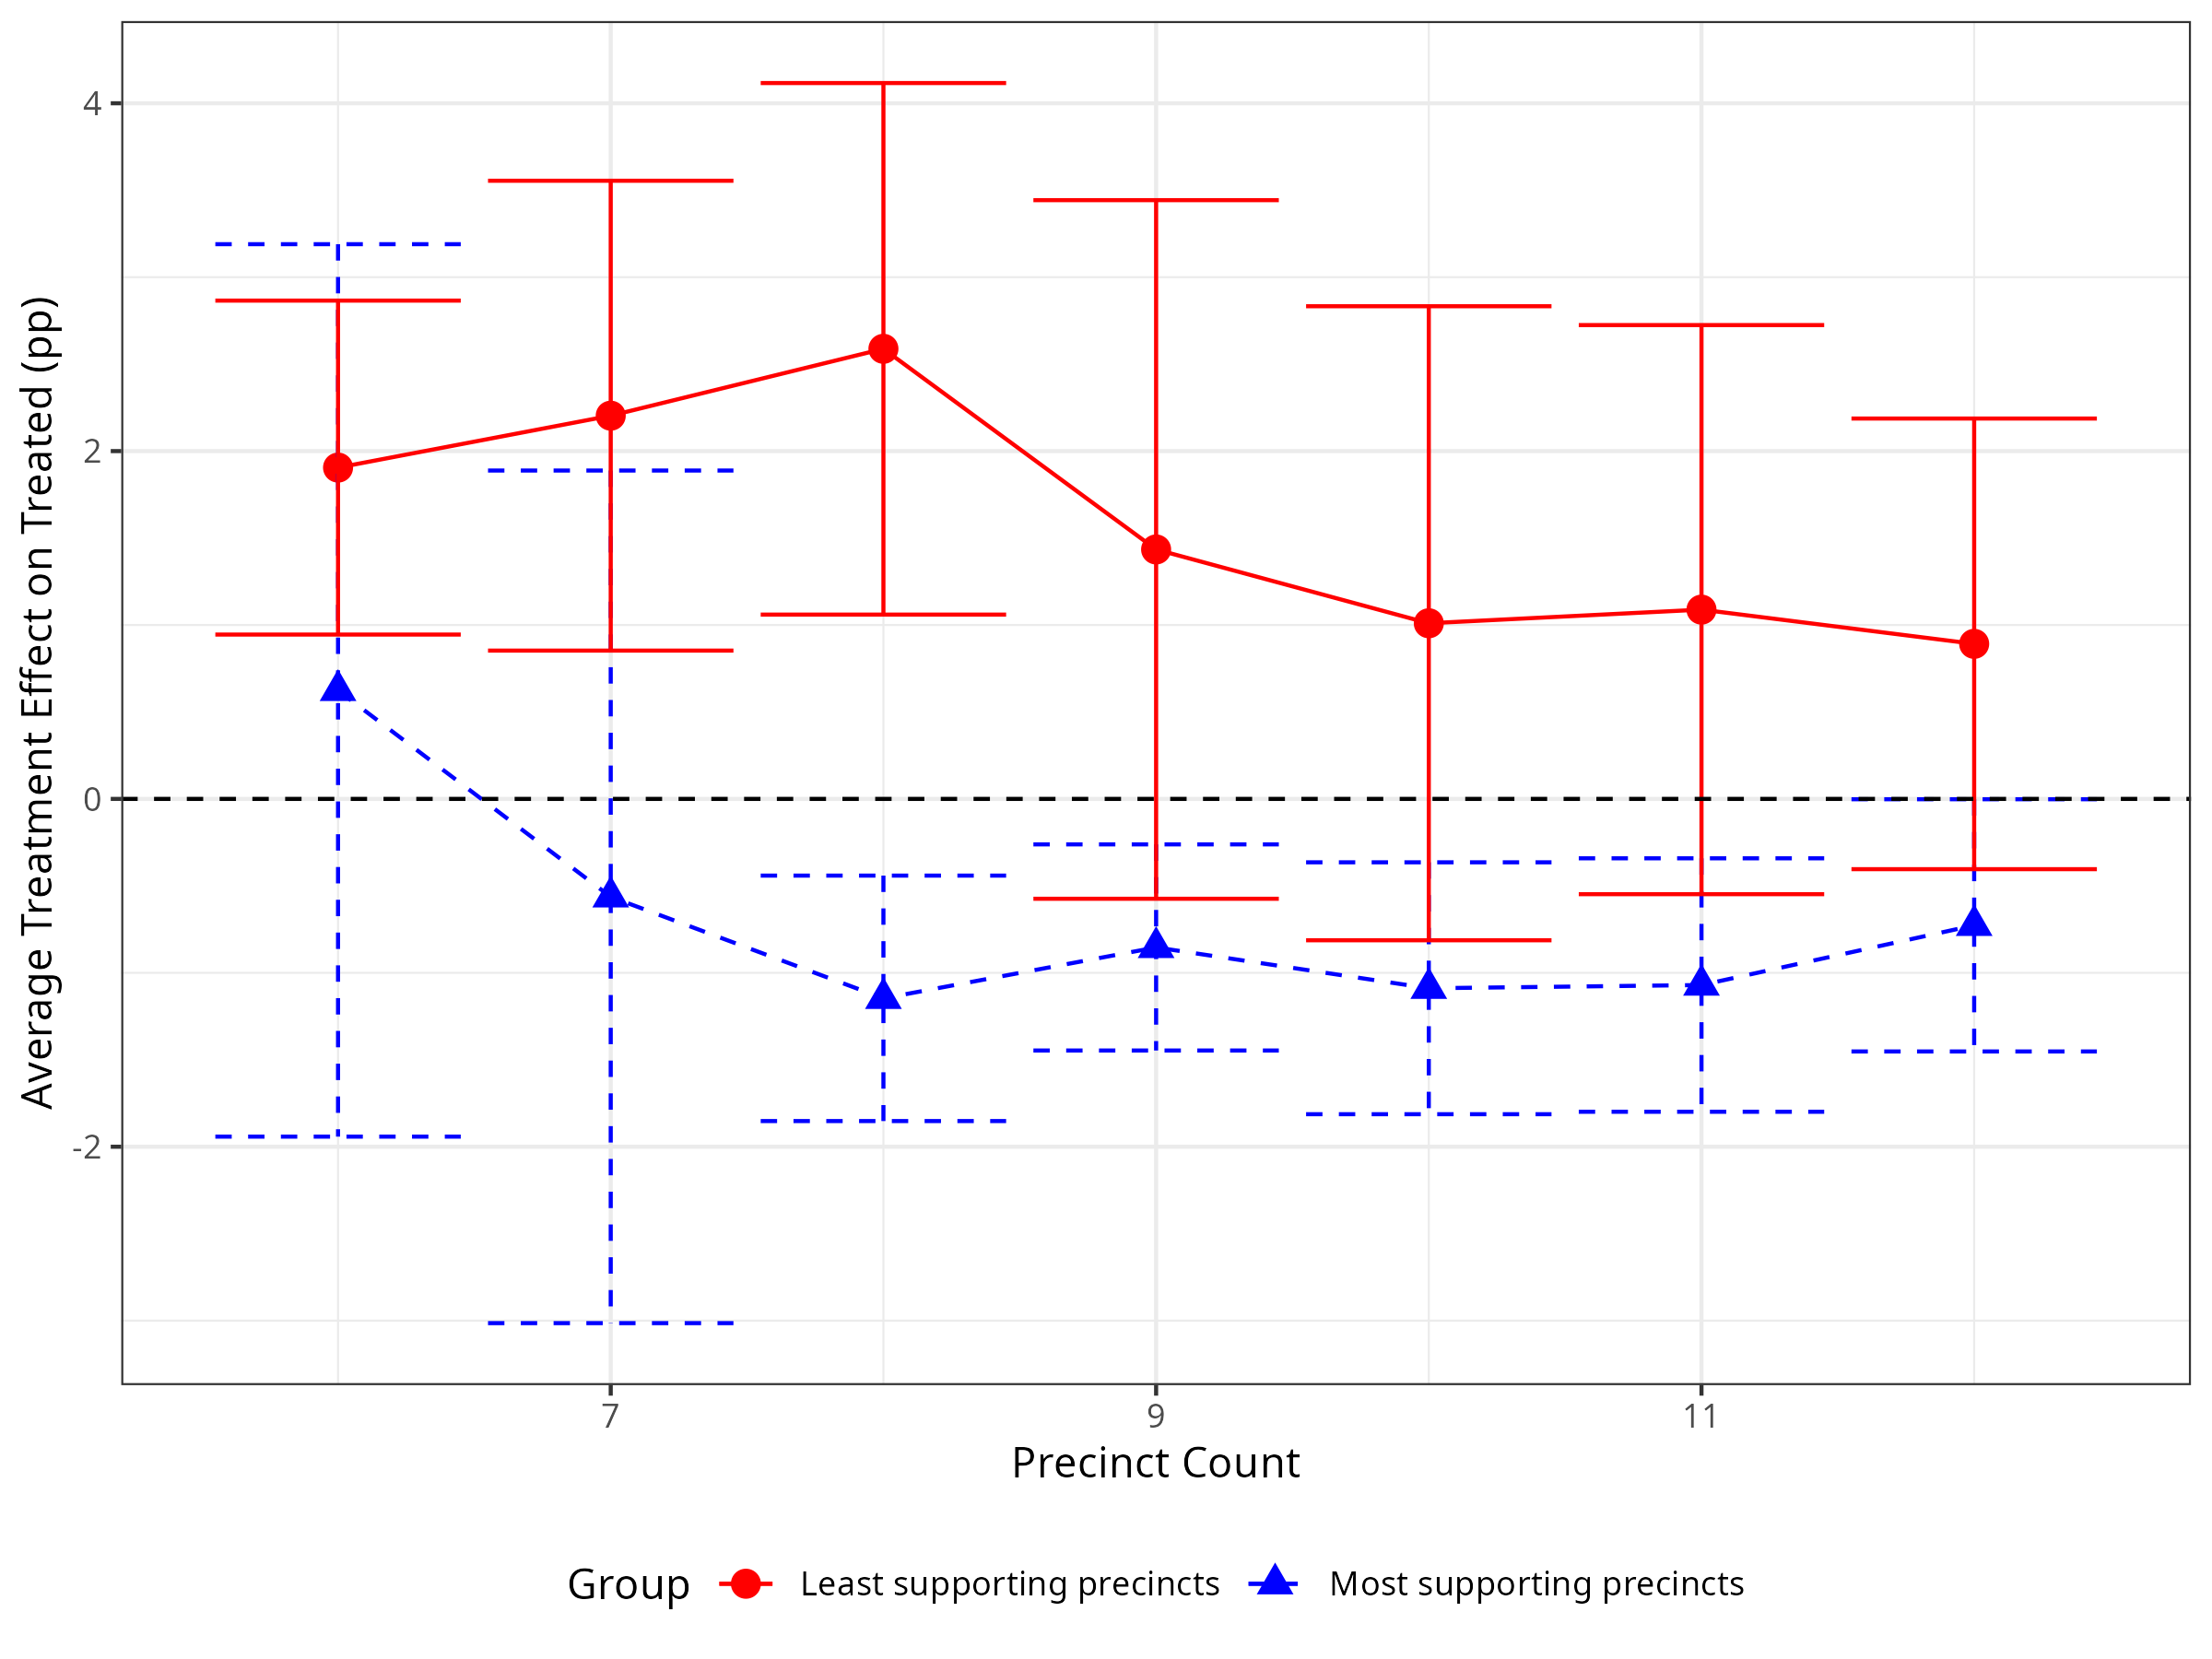
\includegraphics[width=\linewidth]{input/corruption_precinct_variation.png}
        \caption{Corruption}
        \label{fig:ATT_over_time:corruption}
    \end{subfigure}\hfill
    \begin{subfigure}{.48\linewidth}
        \centering
        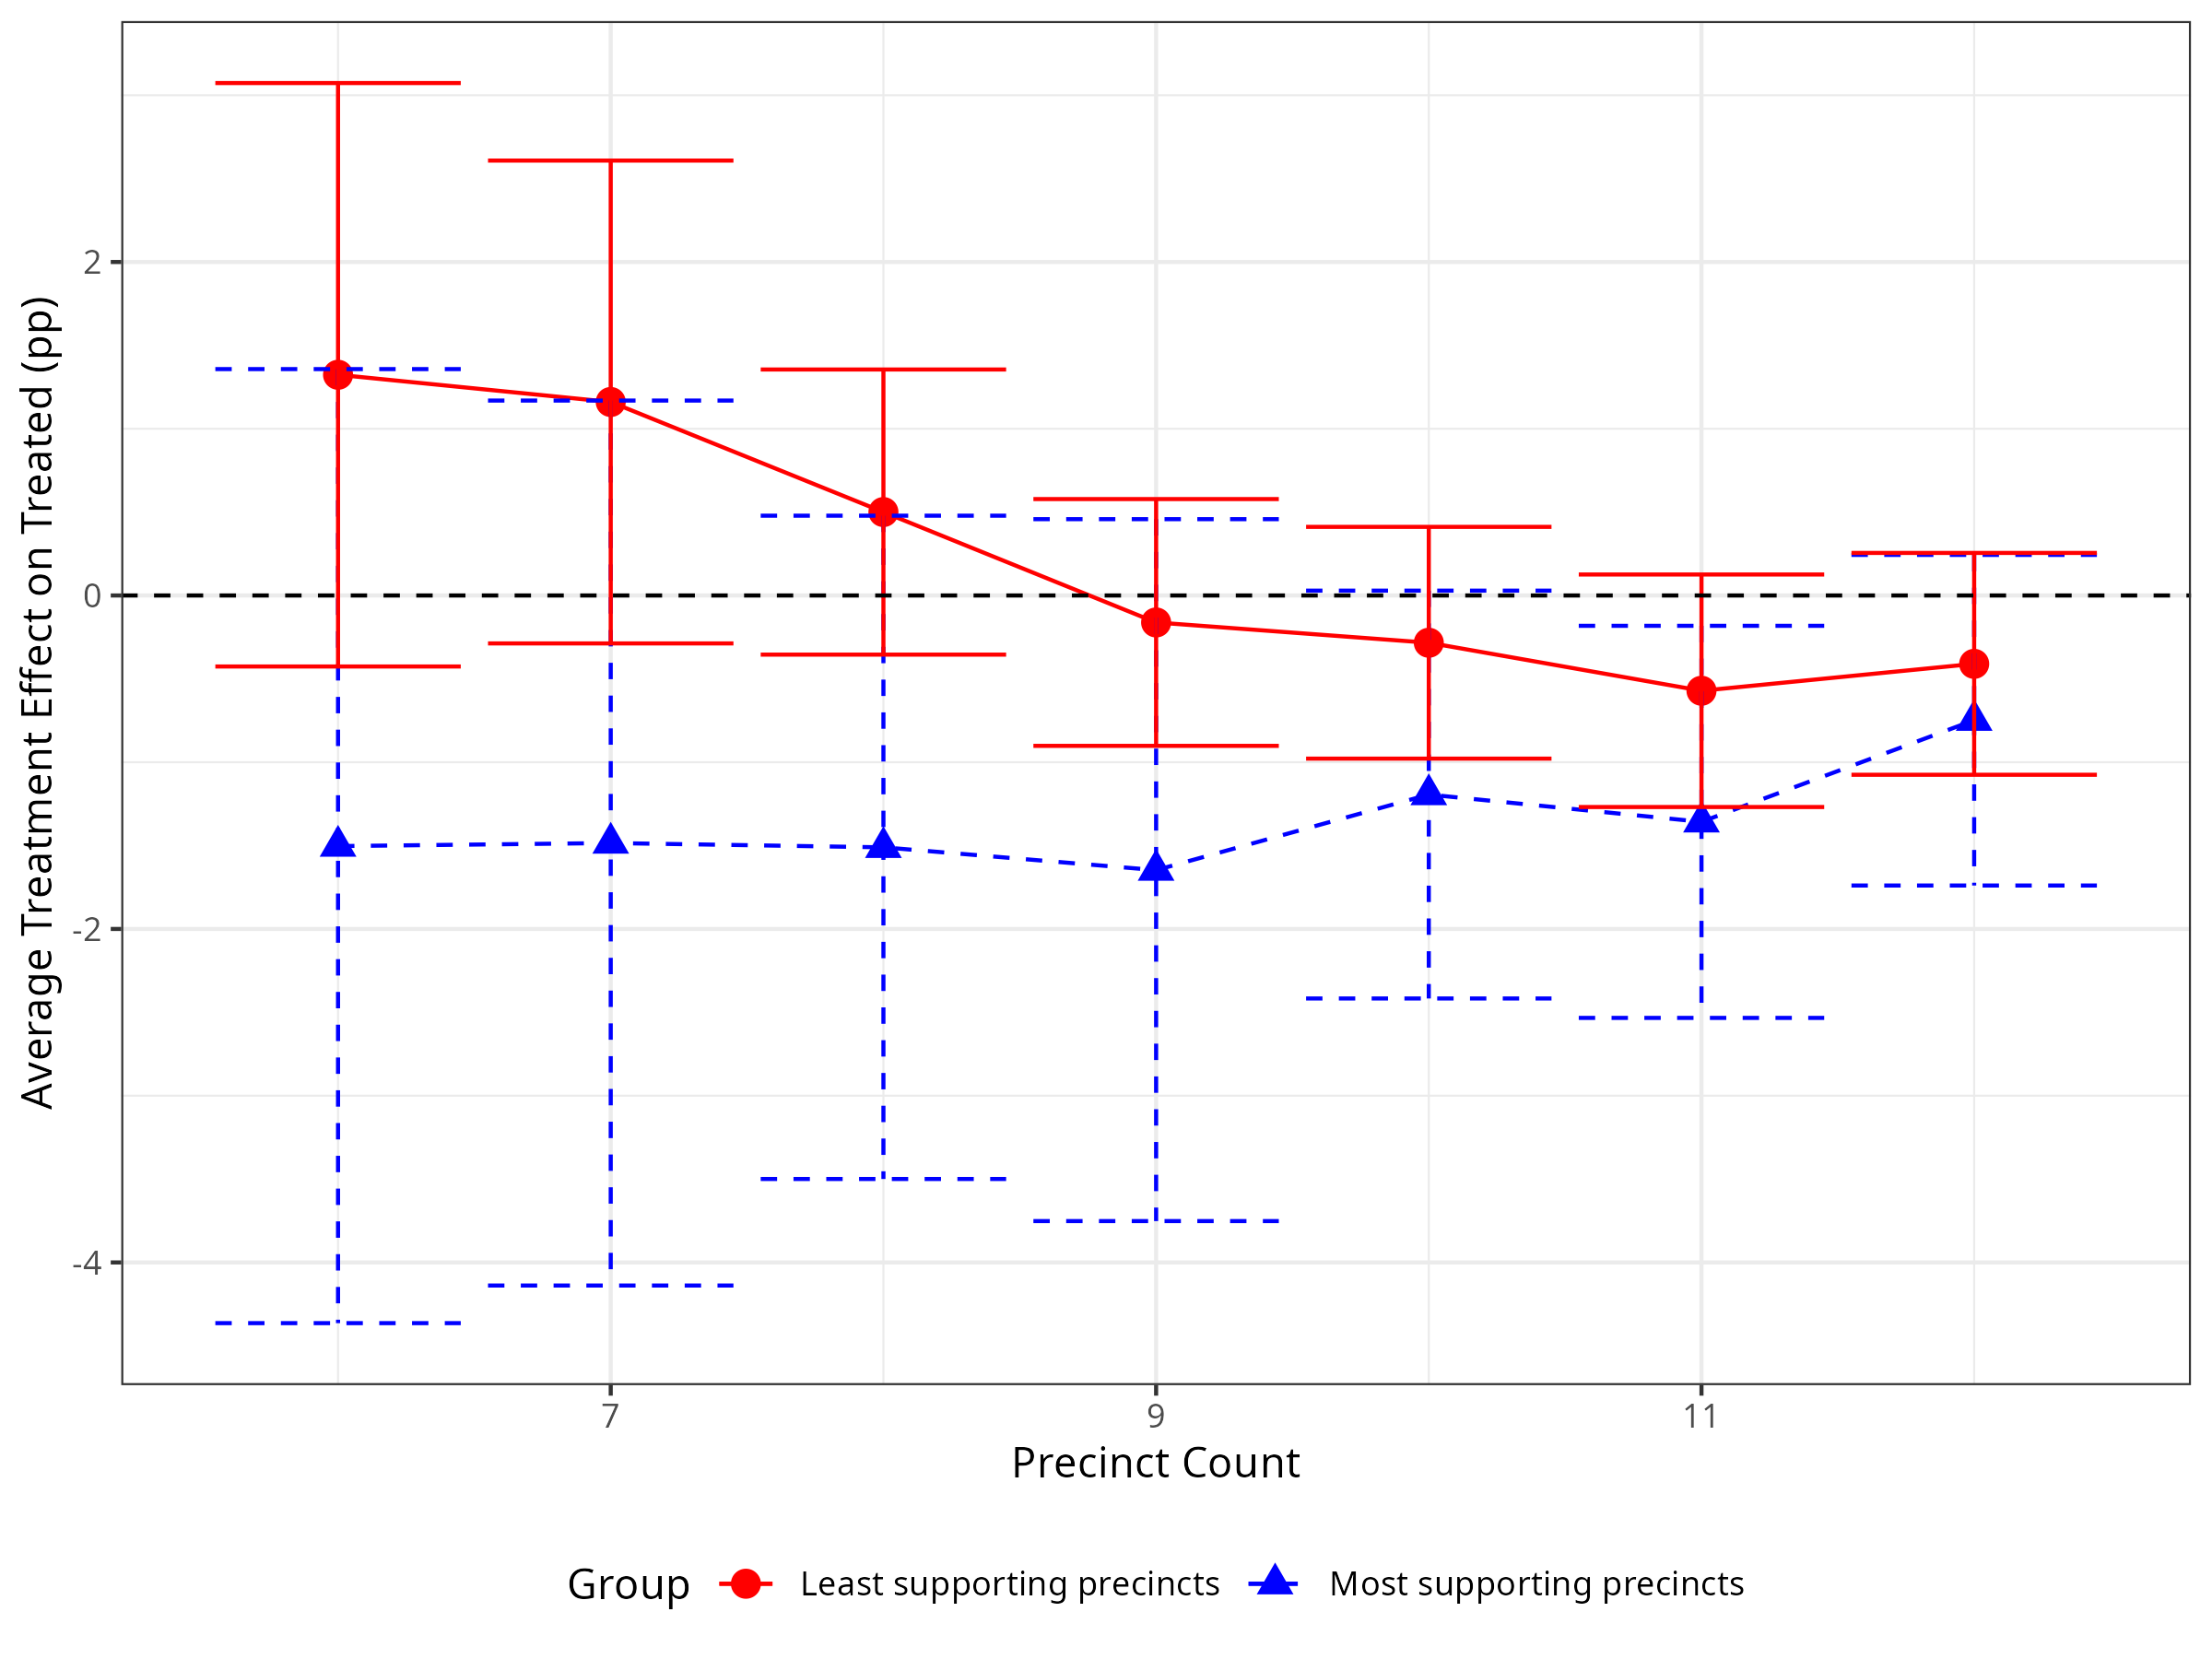
\includegraphics[width=\linewidth]{input/close_elections_precinct_variation.png}
        \caption{Close Election}
        \label{fig:ATT_across_precincts:close_election}
    \end{subfigure}
\end{figure}
\section*{Conclusions}\label{sec:conclusions}

Overall we find some evidence that aldermen may sometimes disproportionately allocate spending to their most supporting precincts, particularly when they are long-entrenched and not facing a competitive election.
The paper starts by verifying a rumor that a particular alderman disproportionately allocated spending to his most supporting precincts.
Then it uses two applications of a differences-in-differences research design to arrive at this fact.
The first application focuses on aldermen who lost by a small margin, and finds that the evidence for disproportionate spending is very weak.
While the magnitude of the estimated effect on the top precincts in the close election design is large, it is not even close to statistically significant, and even the sign of the effect is not robust to changes in the number of supporting/opposing precincts included in the sample.
We find that the effect is economically large and statistically significant when we use the indictment design.
The statistical significance is sensitive to parameters such as the number of supporting or opposing precincts included per ward, but the economic significance is not and stays largely the same for this design so long as you decrease the number of precincts.
This is likely due to the fact that increasing the number of precincts dilutes the average treatment effect, so it decreases the aggregated treatment effect.

The results help build on the burgeoning urban economics of infrastructure literature by showing that political incentives can distort the allocation of infrastructure spending.
Secondly, the differences between the competitive election and indictment designs show that the electoral competition can be a powerful force in constraining the clientelistic tendencies of politicians.
There is also a lesson in urban planners that while discretion can be useful, it can also be abused and lead to unintended consequences.
Therefore, the capacity for discretion should be carefully considered when designing a program.


% -----------------------------------------------
% 	REFERENCES
% -----------------------------------------------

\bibliography{../bib/machine.bib}{}

\newpage
\clearpage

% \begin{center} \Large \textbf{Appendix -- For Online Publication} \end{center}
% \appendix
% \numberwithin{equation}{section}
% \numberwithin{figure}{section}
% \numberwithin{table}{section}

% \section*{Appendix: Regression Results with Beautification}

\begin{table}[H] \centering 
  \caption{Discrete Choice and TWFE results with Beautification} 
  \label{} 
\begin{tabular}{lccc} 
\\[-1.8ex]\hline 
\hline \\[-1.8ex] 
 & \multicolumn{3}{c}{\textit{Model:}} \\ 
\cline{2-4} 
\\[-1.8ex] & Discrete Choice & OLS & Experience OLS \\ 
\\[-1.8ex] & (1) & (2) & (3)\\ 
\hline \\[-1.8ex] 
 beauty & 0.281$^{**}$ & 6.690$^{**}$ & 5.696$^{*}$ \\ 
  & (0.119) & (2.770) & (2.833) \\ 
  & & & \\ 
 exp &  &  & $-$0.447 \\ 
  &  &  & (0.343) \\ 
  & & & \\ 
 Constant & $-$0.941$^{*}$ & 27.667$^{**}$ & 33.379$^{**}$ \\ 
  & (0.532) & (12.345) & (12.928) \\ 
  & & & \\ 
\hline \\[-1.8ex] 
Observations & 71 & 71 & 71 \\ 
R$^{2}$ & 0.863 & 0.846 & 0.857 \\ 
Adjusted R$^{2}$ & 0.583 & 0.532 & 0.546 \\ 
Residual Std. Error & 0.329 (df = 23) & 7.643 (df = 23) & 7.530 (df = 22) \\ 
F Statistic & 3.078$^{***}$ (df = 47; 23) & 2.696$^{***}$ (df = 47; 23) & 2.755$^{***}$ (df = 48; 22) \\ 
\hline 
\hline \\[-1.8ex] 
\textit{Note:}  & \multicolumn{3}{r}{$^{*}$p$<$0.1; $^{**}$p$<$0.05; $^{***}$p$<$0.01} \\ 
\end{tabular} 
\end{table} 


\begin{table}[H] \centering 
  \caption{OLS Results with Unopposed Candidates Included} 
  \label{} 
\begin{tabular}{@{\extracolsep{5pt}}lcc} 
\\[-1.8ex]\hline 
\hline \\[-1.8ex] 
 & \multicolumn{2}{c}{\textit{Dependent variable:}} \\ 
\cline{2-3} 
\\[-1.8ex] & \multicolumn{2}{c}{Vote Share} \\ 
\\[-1.8ex] & (1) & (2)\\ 
\hline \\[-1.8ex] 
 off\_menu & 4.918 &  \\ 
  & (3.654) &  \\ 
  & & \\ 
 exp &  & $-$0.949 \\ 
  &  & (0.626) \\ 
  & & \\ 
 Constant & 32.639 & 55.827$^{***}$ \\ 
  & (20.171) & (15.028) \\ 
  & & \\ 
\hline \\[-1.8ex] 
Observations & 83 & 83 \\ 
R$^{2}$ & 0.727 & 0.731 \\ 
Adjusted R$^{2}$ & 0.301 & 0.311 \\ 
Residual Std. Error (df = 32) & 14.804 & 14.699 \\ 
F Statistic (df = 50; 32) & 1.705$^{*}$ & 1.739$^{**}$ \\ 
\hline 
\hline \\[-1.8ex] 
\textit{Note:}  & \multicolumn{2}{r}{$^{*}$p$<$0.1; $^{**}$p$<$0.05; $^{***}$p$<$0.01} \\ 
\end{tabular} 
\end{table} 



% Table created by stargazer v.5.2.3 by Marek Hlavac, Social Policy Institute. E-mail: marek.hlavac at gmail.com
% Date and time: Tue, Jan 24, 2023 - 08:33:57 PM
\begin{table}[H] \centering 
  \caption{Regression Discontinuity Results with Beautification} 
  \label{rdd_cutoff_table_beauty} 
\small 
\begin{tabular}{@{\extracolsep{0pt}}lcccc} 
\\[-1.8ex]\hline 
\hline \\[-1.8ex] 
 & \multicolumn{4}{c}{Bandwidth Criterion:} \\ 
\cline{2-5} 
\\[-1.8ex] & \multicolumn{4}{c}{beauty} \\ 
 & Full & IK & MSE & CER \\ 
\\[-1.8ex] & (1) & (2) & (3) & (4)\\ 
\hline \\[-1.8ex] 
 IW & 397 & 251 & 253 & 524 \\ 
  & (6,577) & (6,874) & (8,428) & (9,127) \\ 
  & & & & \\ 
 IVS & $-$2,016 & $-$2,016 & $-$7,480 & $-$37,940 \\ 
  & (75,033) & (75,044) & (237,448) & (342,903) \\ 
  & & & & \\ 
 IW:IVS & 1,930 & 3,542 & 11,355 & 44,949 \\ 
  & (75,725) & (79,608) & (243,401) & (354,017) \\ 
  & & & & \\ 
 Constant & 49,575$^{***}$ & 49,575$^{***}$ & 49,450$^{***}$ & 49,090$^{***}$ \\ 
  & (6,077) & (6,078) & (7,567) & (8,113) \\ 
  & & & & \\ 
\hline \\[-1.8ex] 
Observations & 4,150 & 3,250 & 2,300 & 1,900 \\ 
R$^{2}$ & 0 & 0 & 0 & 0 \\ 
Adjusted R$^{2}$ & $-$0 & $-$0 & $-$0 & $-$0 \\ 
Residual Std. Error & 103,521 (df = 4146) & 103,536 (df = 3246) & 103,532 (df = 2296) & 103,546 (df = 1896) \\ 
F Statistic & 0 (df = 3; 4146) & 0 (df = 3; 3246) & 0 (df = 3; 2296) & 0 (df = 3; 1896) \\ 
\hline 
\hline \\[-1.8ex] 
\textit{Note:}  & \multicolumn{4}{r}{$^{*}$p$<$0.1; $^{**}$p$<$0.05; $^{***}$p$<$0.01} \\ 
\end{tabular} 
\end{table} 


% Table created by stargazer v.5.2.3 by Marek Hlavac, Social Policy Institute. E-mail: marek.hlavac at gmail.com
% Date and time: Sun, Jul 17, 2022 - 03:52:33 PM
\begin{table}[H] \centering 
  \caption{Diff-in-Diff Results with Beautification} 
  \label{} 
\begin{tabular}{@{\extracolsep{5pt}}lccc} 
\\[-1.8ex]\hline 
\hline \\[-1.8ex] 
 & \multicolumn{3}{c}{\textit{Treatment Variable:}} \\ 
\cline{2-4} 
\\
\\[-1.8ex] & Both & Electoral Only & Retirement Only\\ 
\hline \\[-1.8ex] 
 treated & 96,202.610$^{***}$ & 105,220.300$^{**}$ & 81,802.030$^{*}$ \\ 
  & (33,413.550) & (41,793.240) & (47,734.510) \\ 
  & & & \\ 
 treated\_1 & $-$50,774.430 & $-$99,109.770$^{*}$ & $-$44,385.510 \\ 
  & (42,265.170) & (59,103.990) & (60,379.910) \\ 
  & & & \\ 
 treated\_2 & 8,470.087 & 33,825.860 & 17,229.070 \\ 
  & (42,265.170) & (59,103.990) & (60,379.910) \\ 
  & & & \\ 
 treated\_3 & $-$30,194.430 & $-$82,640.400 & 1,600.154 \\ 
  & (42,265.170) & (59,103.990) & (60,379.910) \\ 
  & & & \\ 
 treated\_4 & 27,918.280 & 27,503.180 & 36,145.330 \\ 
  & (42,265.170) & (59,103.990) & (60,379.910) \\ 
  & & & \\ 
 Constant & 297,785.700$^{***}$ & 56,001.950$^{***}$ & 298,376.600$^{***}$ \\ 
  & (32,512.140) & (18,688.580) & (32,644.510) \\ 
  & & & \\ 
\hline \\[-1.8ex] 
Observations & 450 & 405 & 378 \\ 
R$^{2}$ & 0.355 & 0.050 & 0.382 \\ 
Adjusted R$^{2}$ & 0.252 & 0.016 & 0.279 \\ 
Residual Std. Error & 90,253.700 (df = 387) & 107,186.800 (df = 390) & 89,606.330 (df = 323) \\ 
F Statistic & 3.440$^{***}$ (df = 62; 387) & 1.466 (df = 14; 390) & 3.696$^{***}$ (df = 54; 323) \\ 
\hline 
\hline \\[-1.8ex] 
\textit{Note:}  & \multicolumn{3}{r}{$^{*}$p$<$0.1; $^{**}$p$<$0.05; $^{***}$p$<$0.01} \\ 
\end{tabular} 
\end{table} 
%\input{./sections/appendix_data.tex}
%\input{./sections/appendix_empirics.tex}

\end{document}